\chapter{低温下的电子序}\label{chap:low-and-super}

由于不同的相互作用通道,凝聚态体系中可以有各种各样的电子凝聚:自旋密度波%
\footnote{
    为了避免引起混淆我们要区分自旋密度波和自旋波。后者是一个自旋系统中的现象,前者是一个费米子系统中的现象。
    或者,更加形象地说,后者是固定在格点上的自旋的空间涨落,前者是可以运动的、携带自旋的费米子密度的空间涨落。
}%
、电荷密度波、超导配对等。
此时的系统不再是一个普通的费米液体了,相互作用改变了系统的元激发谱,我们也可以说,\emph{特殊的相互作用通道让费米液体不稳定}。
超导配对顾名思义,可能导致可以不受阻碍地随意移动的“超导电子”出现;所谓密度波实际上就是一种长程序,它在空间中有一种周期性振荡,可以是相位的振荡也可以是大小的振荡,
也即,这样的长程序对应的序参量形如
\begin{equation}
    \Delta(\vb*{r}) \sim \Delta_0 \ee^{\ii \vb*{Q} \cdot \vb*{r}}.
\end{equation}

请注意这个序参量实际上是一种二电子集体运动模式,即相邻的两个电子的自旋总是保持一上一下的这种运动模式。
这暗示我们,如果需要超越平均场近似的理论,只需要把这种模式定义成一个新的(玻色)场就可以。
本节讨论的这些现象对应的序参量均对应于Hubbard-Stratonovich参量(见\autoref{back:gl-hubbard-stratonovich})的不同选择,即我们只讨论序参量能够写成两个电子场乘积的线性组合的那些序。
更加物理地说,我们只讨论那些在对称性自发破缺发生之后,仍然有普通电子的系统,只不过这些电子受到由于对称性自发破缺,一些电子形成序而产生的较低对称性的势场的作用,能谱发生改变。
相互作用电子体系中的不同的相互作用通道对应不同的Hubbard-Stratonovich参量。
写出这些参量的场论后,我们会发现可能有多个参量都有对称性自发破缺,它们相互竞争,最终哪一种参量最终发生凝聚——从而,单单考虑它得到的相变出现——取决于很多条件。

这个图像并不能覆盖所有相变。例如在

\section{BCS超导}\label{sec:bcs-theory}

本节介绍一种常见的超导机制,即交换声子导致电子出现有效吸引相互作用而产生的BCS超导。
我们将主要讨论所谓的s波超导,其具体含义后面会提到。

\subsection{交换声子导致的有效电子吸引相互作用}\label{sec:phonon-caused-interaction}

\subsubsection{声子介导的电子-电子相互作用}

电子-声子相互作用的顶角为一个电子入射,一个电子出射,产生/消灭一个声子。
现在尝试积掉声子。我们先将电子场当成给定的,则可以从\eqref{eq:simple-phonon-electron-int}写出声子场加上电子-声子相互作用的虚时间作用量。本节仅考虑晶格是简单正方晶格的情况,于是没有各向异性,我们有(关于$\tau$的傅里叶变换见\eqref{eq:imaginary-fourier})
\[
    \begin{aligned}
        S_\text{ph} + S_\text{int} &= \int \dd{\tau} \sum_{\vb*{q}, \lambda} \Big(
        \bar{\phi}_{\vb*{q} \lambda} (\partial_\tau + \omega_{\vb*{q} \lambda}) \phi_{\vb*{q} \lambda}
        + \gamma \frac{\ii q_\lambda}{\sqrt{2 N M \omega_{\vb*{q} \lambda}}} (\phi_{\vb*{q} \lambda} + \bar{\phi}_{-\vb*{q} \lambda}) \underbrace{\sum_{\vb*{k}, \sigma} \bar{\psi}_{(\vb*{k} + \vb*{q}) \sigma} \psi_{\vb*{k} \sigma}}_{\rho_{\vb*{q}}}
        \Big) \\
        &= \sum_{{q}, \lambda} \Big(
            \bar{\phi}_{{q} \lambda} (- \ii \omega_n + \omega_{\vb*{q} \lambda}) \phi_{{q} \lambda}
            + \gamma \frac{\ii \vb*{q} \cdot \vu*{\lambda}}{\sqrt{2 \beta N M \omega_{\vb*{q} \lambda}}} (\phi_{{q} \lambda} + \bar{\phi}_{-{q} \lambda}) \sum_{{k}, \sigma} \bar{\psi}_{({k} + {q}) \sigma} \psi_{{k} \sigma}
        \Big)
    \end{aligned}
\]
其中$\phi$表示声子,$\psi$表示电子,$M$是原子质量。使用处理自由场受到线性激励的方法,配平方并积掉二次方项,忽略产生的因子,得到
\begin{equation}
    \begin{aligned}
        S_\text{eff} &= - \sum_{\omega_n, \vb*{q}, \lambda} \frac{\gamma^2 \abs*{\vb*{q}}^2 \rho_{{q}} \rho_{-{q}}}{2 \beta N M \omega_{\vb*{q} \lambda} (\omega_{\vb*{q} \lambda} - \ii \omega_n)} 
        = - \sum_{\omega_n, \vb*{q}, \lambda} \frac{\gamma^2 \abs*{\vb*{q}}^2 \rho_{{q}} \rho_{-{q}}}{2 \beta N M (\omega_{\vb*{q} \lambda}^2 + \omega_n^2)} \\ 
        &= - \frac{\gamma^2}{2 \beta N M} \sum_{\omega_n, \vb*{q}, {k}, {k}', \alpha, \beta} \frac{\abs*{\vb*{q}}^2}{\omega_n^2 + \omega_{\vb*{q} \lambda}^2} \bar{\psi}_{({k}+{q}) \alpha} \bar{\psi}_{({k}' - {q}) \beta} \psi_{{k}' \beta} \psi_{{k} \alpha} .
    \end{aligned}
    \label{eq:retarded-two-electron}
\end{equation}
第二个等号是考虑到每个$\omega_n$有一个对应的$-\omega_n$而得到的。总之,电子之间可以通过交换声子来产生一个四电子相互作用。
相互作用\eqref{eq:retarded-two-electron}是推迟相互作用,因此原则上不能够仅仅使用一个哈密顿量描述。
不过,在推迟不明显时我们还是可以近似写出一个哈密顿量。这里有一个微妙的地方:\eqref{eq:retarded-two-electron}是定义在虚时间下的,即算符的时间演化为$\ee^{\omega t}$,而我们需要一个实时间下的哈密顿量,所以需要首先做频率上的Wick转动$\omega = \ii \omega_n$(但是另一方面作用量形式上仍然是虚时间场论的作用量,即作用量和哈密顿量之间不相差负号),得到
\[
    S_\text{eff} = - \frac{\gamma^2}{2 \beta N M} \sum_{\omega} \sum_{\vb*{q}, \vb*{k}, \vb*{k}', \alpha, \beta} \frac{\abs*{\vb*{q}}^2}{- \omega^2 + \omega_{\vb*{q} \lambda}^2} \bar{\psi}_{({k}+{q}) \alpha} \bar{\psi}_{({k}' - {q}) \beta} \psi_{{k}' \beta} \psi_{{k} \alpha}.
\]
上式中的所有$\psi$都是$\omega$的函数,可以将它们转换到时域,这将给出一个有推迟的作用量,从而不能简单地用一个哈密顿量描述电子-电子等效相互作用。
上式的无推迟近似是它的无时间变化的傅里叶分量。
因此实际上我们只需要简单地取
\begin{equation}
    \omega = \epsilon_{\vb*{k}} - \epsilon_{\vb*{k} + \vb*{q}},
    \label{eq:phonon-introduced-omega}
\end{equation}
就得到了无推迟的近似%
\footnote{
    通过简单地将
    \[
        \sum_{k, k', q} f(q^0, \vb*{q}) \bar{c}_{k+q} \bar{c}_{k'-q} c_{k'} c_k
    \]
    变换到虚时间时域就可以看出为什么作用量中耦合系数显含$q^0$会导致推迟相互作用,以及为什么取\eqref{eq:phonon-introduced-omega}就给出了这个推迟相互作用的瞬时近似。下同。
}%
\begin{equation}
    \begin{aligned}
        {H} &= - \frac{\gamma^2}{2 N M} \sum_{\vb*{q}, \vb*{k}, \vb*{k}', \alpha, \beta} \frac{\abs*{\vb*{q}}^2}{- \omega^2 + \omega_{\vb*{q} \lambda}^2} {c}^\dagger_{(\vb*{k}+\vb*{q}) \alpha} {c}^\dagger_{(\vb*{k}' - \vb*{q}) \beta} {c}_{\vb*{k}' \beta} {c}_{\vb*{k} \alpha} \\
        &= \frac{\gamma^2}{2 N M} \sum_{\vb*{q}, \vb*{k}, \vb*{k}', \alpha, \beta} \frac{\abs*{\vb*{q}}^2}{(\epsilon_{\vb*{k}} - \epsilon_{\vb*{k}+\vb*{q}})^2 - \omega_{\vb*{q} \lambda}^2} {c}^\dagger_{(\vb*{k}+\vb*{q}) \alpha} {c}^\dagger_{(\vb*{k}' - \vb*{q}) \beta} {c}_{\vb*{k}' \beta} {c}_{\vb*{k} \alpha}.
    \end{aligned}
\end{equation}
应注意,在不采取无推迟相互作用的近似时,关于$\omega$我们仍然有能量守恒关系,但此时我们有的是
\[
    \omega = k^0 - (k + q)^0,
\]
这是关于离壳的虚频率的能量守恒,而不是像\eqref{eq:phonon-introduced-omega}这样的在壳的能量守恒。

更加一般地,设声子频率为$\omega_{\vb*{q}}$,电子-声子相互作用为
\begin{equation}
    H = \frac{1}{\sqrt{N}} \sum_{\vb*{k}, \vb*{q}, \lambda} M_{\vb*{q} \lambda} c^\dagger_{\vb*{k} + \vb*{q}} c_{\vb*{k}} (b_{\vb*{q} \lambda} + b_{-\vb*{q} \lambda}^\dagger),
\end{equation}
由厄米性,有
\begin{equation}
    M_{-\vb*{q} \lambda} = M^*_{\vb*{q} \lambda}.
\end{equation}
重复以上步骤,频域下(动量空间加松原频率)的作用量是
\begin{equation}
    S = \sum_{q, \lambda} \bar{b}_{q \lambda} (- \ii q^0 + \omega_{\vb*{q} \lambda}) b_{q \lambda} + \frac{1}{\sqrt{\beta N}} \sum_{k, q, \lambda} M_{\vb*{q}} \bar{c}_{k + q} c_{k} (b_{q \lambda} + \bar{b}_{- q \lambda}),
    \label{eq:bcs-original-action-freq}
\end{equation}
利用高斯积分
\[
    \int \dd{(x, x^\dagger)} \ee^{x^\dagger A x + b^\dagger x + x^\dagger b} \simeq \ee^{- b^\dagger A b},
\]
积掉声子自由度,得到
\begin{equation}
    \begin{aligned}
        S_\text{eff} &= - \frac{1}{\beta N} \sum_{q, \lambda} M_{\vb*{q} \lambda} \sum_{k, \sigma} \bar{c}_{k+q, \sigma} c_{k \sigma} \frac{1}{- \ii q^0 + \omega_{\vb*{q} \lambda}} M_{- \vb*{q} \lambda} \sum_{k', \sigma'} \bar{c}_{k' - q, \sigma'} c_{k' \sigma'} \\
        &= - \frac{1}{\beta N} \sum_{q, \lambda} M_{\vb*{q} \lambda} \sum_{k, \sigma} \bar{c}_{k+q, \sigma} c_{k \sigma} \frac{1}{2} \left( \frac{1}{- \ii q^0 + \omega_{\vb*{q} \lambda}} + \frac{1}{\ii q^0 + \omega_{\vb*{q} \lambda}} \right) M_{- \vb*{q} \lambda} \sum_{k', \sigma'} \bar{c}_{k' - q, \sigma'} c_{k' \sigma'} \\
        &= - \frac{1}{\beta N} \sum_{q, \lambda} \sum_{k, k', \alpha, \beta} \abs*{M_{\vb*{q}}}^2 \frac{\omega_{\vb*{q} \lambda}}{\omega_{\vb*{q} \lambda}^2 + (q^0)^2} \bar{c}_{k + q, \alpha} \bar{c}_{k' - q, \beta} c_{k' \beta} c_{k \alpha}.
    \end{aligned}
    \label{eq:integrating-out-phonon}
\end{equation}
Wick转动会让$\ii q^0$变成$\omega$。注意$c_{k \alpha}$这些算符中的$k^0$未必是$\epsilon_{\vb*{k}}$。将上式切换回到频域,得到的是推迟相互作用。
然而实际上晶格存在各种弛豫机制,声子被一个电子产生之后不可能维持特别长的时间再和另一个电子散射。在前面的推导中我们没有将声子弛豫体现出来,但是声子的寿命有限这件事让推迟相互作用的时间延迟有一个截断。
因此我们仅仅考虑上式中那些瞬时发生的相互作用通道,为此必须让相互作用耦合系数没有任何$k^0, k^{'0}, q^0$的依赖,因此我们只考虑最重要的
\begin{equation}
    \omega = \epsilon_{\vb*{k}} - \epsilon_{\vb*{k}+\vb*{q}},
\end{equation}
切换到时域得到
\begin{equation}
    {H}_{4\text{e}} = \frac{1}{2N} \sum_{\vb*{k}, \vb*{k}', \vb*{q}'} \sum_{\alpha, \beta} \abs{M_{\vb*{q}}}^2 \frac{\omega_{\vb*{q} \lambda}}{(\epsilon_{\vb*{k}} - \epsilon_{\vb*{k}+\vb*{q}})^2 - \omega_{\vb*{q}}^2} {c}^\dagger_{(\vb*{k}+\vb*{q}) \alpha} {c}^\dagger_{(\vb*{k}'-\vb*{q}) \beta} {c}_{\vb*{k}' \beta} {c}_{\vb*{k} \alpha}.
    \label{eq:4-electron-interaction-by-phonon}
\end{equation}

在只考虑二声子一电子的相互作用顶角时,任何更复杂的含有声子的费曼图都可以化归为二电子和声子的相互作用和一些电子相互作用的组合,因此\eqref{eq:4-electron-interaction-by-phonon}就给出了完整的没有声子的有效理论。
\eqref{eq:4-electron-interaction-by-phonon}本身是瞬时的,但即使我们不知道它来自一个推迟相互作用,\eqref{eq:4-electron-interaction-by-phonon}含有电子能量差而\eqref{eq:phonon-introduced-omega}也有这一事实也暗示它有可能实际上代表一个推迟相互作用。
另一方面,库伦势则没有推迟(当然这实际上做了近似,我们只不过不考虑相对论效应而已,但是电磁相互作用的推迟远小于声子传递导致的推迟)。

在以上推导过程中应当注意一点:我们在这里使用的实际上不是标准的声子传播子。\eqref{eq:bcs-original-action-freq}中的声子自由部分是直接根据声子哈密顿量(类似于\eqref{eq:1d-phonon-ham})写出来的,
在此过程中我们\emph{没有}考虑产生声子的场是实场这件事,而是将$b_{\vb*{q} \lambda}$傅里叶变换到实空间中的结果当成了产生声子的场,而这显然是一个复场。
因此,在作用量\eqref{eq:bcs-original-action-freq}中,积掉声子得到的有效电子-电子作用量不需要乘以$1/2$。
更加常见的,声子传播子会被写成
\[
    \frac{\ii 2 \omega_{\vb*{q}}}{\omega^2 - \omega_{\vb*{q}}^2 + \ii 0^+},
\]
这个传播子实际上是$\phi_{q \lambda} + \bar{\phi}_{-q, \lambda}$的格林函数,即我们将声子的产生湮灭算符打包成了一个实场,此时纯声子的作用量中将会出现$\omega$的二次项以及一个$1/2$因子,而电子-声子相互作用顶角将只有一个,此时的高斯积分是
\[
    \int \dd{x} \ee^{ \frac{1}{2} x A x + b x} \simeq \ee^{- \frac{1}{2} b A b},
\]
于是\eqref{eq:integrating-out-phonon}的第一行将会变成
\[
    \frac{1}{2} \frac{2 \omega_{\vb*{q} \lambda}}{(q^0)^2 + \omega_{\vb*{q} \lambda}^2},
\]
最终结果完全一致。注意,无论是实场还是复场,$q^0$都可以取负值。

\subsubsection{费米球附近的过程}

现在考虑\eqref{eq:4-electron-interaction-by-phonon}的低能有效理论,其中我们需要考虑的过程全部发生在费米面附近,入射电子和出射电子能量都接近于$\epsilon_\text{F}$。
费米面是球形的,通过几何关系可以看出$\vb*{k} + \vb*{k}' = 0$的过程是最重要的。
如果$\vb*{k}$和$\vb*{k}'$是两个任意的动量,那么动量守恒加上电子在费米面附近的条件意味着可能的出射态是非常小的,但是如果$\vb*{k} + \vb*{k}' = 0$,那么可能的出射态遍布整个费米面。
因此可以判断,$\vb*{k} + \vb*{k}' = 0$的相互作用通道是最重要的相互作用通道。
这样\eqref{eq:4-electron-interaction-by-phonon}就简化为
\begin{equation}
    {H}_{4\text{e}} = \frac{1}{2N} \sum_{\vb*{k}, \vb*{q}'} \underbrace{\sum_{\alpha, \beta} \abs{M_{\vb*{q}}}^2 \frac{\omega_{\vb*{q}}}{(\epsilon_{\vb*{k}} - \epsilon_{\vb*{k}+\vb*{q}})^2 - \omega_{\vb*{q}}^2}}_{V(\vb*{q}, \epsilon_{\vb*{k}} - \epsilon_{\vb*{k}+\vb*{q}})} {c}^\dagger_{(\vb*{k}+\vb*{q}) \alpha} {c}^\dagger_{(-\vb*{k}-\vb*{q}) \beta} {c}_{-\vb*{k} \beta} {c}_{\vb*{k} \alpha}.
    \label{eq:low-energy-4-electron}
\end{equation}
由于电子能量差非常小,显然
\[
    V(\vb*{q}, \epsilon_{\vb*{k}} - \epsilon_{\vb*{k}+\vb*{q}}) = \abs{M_{\vb*{q}}}^2 \frac{\omega_{\vb*{q}}}{(\epsilon_{\vb*{k}} - \epsilon_{\vb*{k}+\vb*{q}})^2 - \omega_{\vb*{q}}^2} < 0,
\]
因此这个声子中介的相互作用是吸引相互作用。

库伦相互作用是排斥的,电-声子相互作用是吸引的;绝对强度显然是前者强。
然而,实际上库伦相互作用很容易被屏蔽,因为把低能电子看成外加电荷,那么高能电子就会来屏蔽它(见\autoref{sec:ext-e}),因此把高能电子积掉之后得到的屏蔽库仑相互作用并不强,因此在重整化下,库仑相互作用实际上只是对电子能带的修正(这和费米液体的想法很相似:渐染地加入一个不大的相互作用仅仅会导致电子自能修正而已)。
另一方面,电-声子相互作用是不容易屏蔽的——\eqref{eq:4-electron-interaction-by-phonon}有一个非常物理的解释:一个电子因为电子-声子散射,在晶格中运行时产生了一列格波,电子很快被散射到别处,但是另一个电子受到先前的那列格波作用,这就建立了长程的电子-电子吸引;实际上推迟相互作用就是不容易屏蔽的。
因此,\eqref{eq:low-energy-4-electron}在重整化之后是主要的电子间相互作用。
还有一种看待这个问题的角度是,电-声子相互作用会导致有效的吸引,在重整化下一个吸引相互作用通常会导致粒子配对取代单粒子自由度成为主要的自由度,因此吸引相互作用不可能只是对能带的修正,而必然导致严重的费米面不稳定;库仑相互作用在这里是排斥的,不会造成粒子配对,因此正如Hartree-Fock近似中的那样,仅仅对电子能级产生了一个修正。

\begin{figure}
    \centering
    

\tikzset{every picture/.style={line width=0.75pt}} %set default line width to 0.75pt        

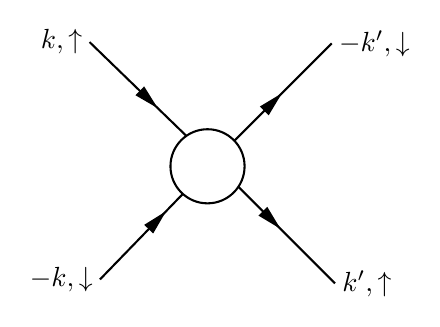
\begin{tikzpicture}[x=0.75pt,y=0.75pt,yscale=-1,xscale=1]
%uncomment if require: \path (0,300); %set diagram left start at 0, and has height of 300

%Straight Lines [id:da749548062064421] 
\draw    (97,121) -- (162.71,184.67) ;
\draw [shift={(129.85,152.84)}, rotate = 224.1] [fill={rgb, 255:red, 0; green, 0; blue, 0 }  ][line width=0.08]  [draw opacity=0] (12,-3) -- (0,0) -- (12,3) -- cycle    ;
%Straight Lines [id:da6891160905390028] 
\draw    (162.71,184.67) -- (215.3,237.27) ;
\draw [shift={(189,210.97)}, rotate = 225] [fill={rgb, 255:red, 0; green, 0; blue, 0 }  ][line width=0.08]  [draw opacity=0] (12,-3) -- (0,0) -- (12,3) -- cycle    ;
%Straight Lines [id:da7275939049575368] 
\draw    (102.03,235.38) -- (165.71,169.67) ;
\draw [shift={(133.87,202.53)}, rotate = 494.1] [fill={rgb, 255:red, 0; green, 0; blue, 0 }  ][line width=0.08]  [draw opacity=0] (12,-3) -- (0,0) -- (12,3) -- cycle    ;
%Straight Lines [id:da3845184529667176] 
\draw    (165.71,169.67) -- (213.71,121.67) ;
\draw [shift={(189.71,145.67)}, rotate = 495] [fill={rgb, 255:red, 0; green, 0; blue, 0 }  ][line width=0.08]  [draw opacity=0] (12,-3) -- (0,0) -- (12,3) -- cycle    ;
%Shape: Circle [id:dp7787521694372523] 
\draw  [fill={rgb, 255:red, 255; green, 255; blue, 255 }  ,fill opacity=1 ] (136,180.85) .. controls (136,170.99) and (143.99,163) .. (153.85,163) .. controls (163.71,163) and (171.71,170.99) .. (171.71,180.85) .. controls (171.71,190.71) and (163.71,198.71) .. (153.85,198.71) .. controls (143.99,198.71) and (136,190.71) .. (136,180.85) -- cycle ;

% Text Node
\draw (95,121) node [anchor=east] [inner sep=0.75pt]    {$\boldsymbol{k} ,\uparrow $};
% Text Node
\draw (100.03,235.38) node [anchor=east] [inner sep=0.75pt]    {$-\boldsymbol{k} ,\downarrow $};
% Text Node
\draw (217.3,237.27) node [anchor=west] [inner sep=0.75pt]    {$\boldsymbol{k} ',\uparrow $};
% Text Node
\draw (215.71,121.67) node [anchor=west] [inner sep=0.75pt]    {$-\boldsymbol{k} ',\downarrow $};


\end{tikzpicture}

    \caption{球形费米面附近最为重要的相互作用通道}
\end{figure}

声子的频率只出现在0和德拜频率$\omega_\text{D}$之间,换而言之吸引相互作用只出现在
\begin{equation}
    \omega = \abs{\epsilon_{\vb*{k}} - \epsilon_{\vb*{k}+\vb*{q}}} < \omega_\text{D}
    \label{eq:bcs-phonon-range}
\end{equation}
时。
数值计算可以表明对超导现象而言最重要的是建立起电子之间的吸引相互作用,其具体形式并不重要,这是因为会参与超导的实际上只有费米面附近的非常小的一个能量范围内的电子,因此$V$的具体形式根本不重要,实际发挥作用的只有费米面上的$V$值。
对本节讨论的球形费米面,在要求\eqref{eq:bcs-phonon-range}实际上就等价于
这样我们设
\begin{equation}
    V(\vb*{q}, \omega) = \begin{cases}
        - V_0, \quad \omega < \omega_\text{D}, \\
        0, \quad \omega > \omega_\text{D}
    \end{cases}.
    \label{eq:superconductive-interaction-simplified}
\end{equation}
其中$\omega_\text{D}$是一个硬截断。这是一个非常粗糙的截断,其合理性在于,由于我们考虑的过程全部发生在费米面附近,在电子动能与费米能量之差普遍不高时,能够激发出来的声子模式能量显然也很低,因此实际上只有声学声子能够被激发,德拜模型适用,这就是为什么我们认为$\omega > \omega_\text{D}$时无有效电子-电子吸引相互作用,因为能够介导这种吸引相互作用的声子根本就不能被激发出来;在$\omega < \omega_\text{D}$时,还是由于电子能量很低,可以用。
这样系统的行为可以通过一个大幅简化的哈密顿量
\begin{equation}
    {H} = \sum_{\vb*{k}, \alpha} (\epsilon_{\vb*{k}} - \mu) {c}_{\vb*{k} \alpha}^\dagger {c}_{\vb*{k} \alpha} - \frac{V_0}{2} \sum_{\vb*{k}, \vb*{q}} \sum_{\alpha, \beta} {c}^\dagger_{(\vb*{k} + \vb*{q}) \alpha} {c}^\dagger_{( - \vb*{k} - \vb*{q}) \beta} {c}_{-\vb*{k} \beta} {c}_{\vb*{k} \alpha}
    \label{eq:simple-super-conductive-hamiltonian}
\end{equation}
加以描述。
$\vb*{k}$和$\vb*{k}+\vb*{q}$都在费米面附近,并且能量相差必须足够小,小于$\omega_\text{D}$。
为了便于做计算,我们仅仅考虑那些这样的$\vb*{k}$和$\vb*{k}+\vb*{q}$:它们都在费米面附近的这样一个区域中,使得从这个区域中任取两个动量$\vb*{k}$和$\vb*{k}'$,它们对应的能量之差的绝对值都小于$\omega_\text{D}$。
由于费米面是球形的,这样一个区域显然由不等式$\xi_\text{min} < \xi_{\vb*{k}} < \xi_\text{max}$确定。
我们是要计算满足对任意$\vb*{k}$和$\vb*{k}'$,均有
\[
    \abs*{\xi_{\vb*{k}} - \xi_{\vb*{k}'}} < \omega_\text{D}
\]
的最大$\xi_{\text{max}}$和最小$\xi_\text{min}$。
简单的计算会表明我们应当取
\[
    \xi_\text{max} = - \xi_\text{min} = \frac{\omega_\text{D}}{2},
\]
即只考虑满足
\begin{equation}
    - \frac{\omega_\text{D}}{2} < \xi_{\vb*{k}} < \frac{\omega_\text{D}}{2}
    \label{eq:bcs-small-sphere-around-fermi-surface}
\end{equation}
的电子模式。
因此以下我们认为\eqref{eq:simple-super-conductive-hamiltonian}仅仅适用于费米面附近宽度为$\omega_\text{D}$的那些电子模式。

\begin{figure}
    \centering
    \tikzset{every picture/.style={line width=0.75pt}} %set default line width to 0.75pt        

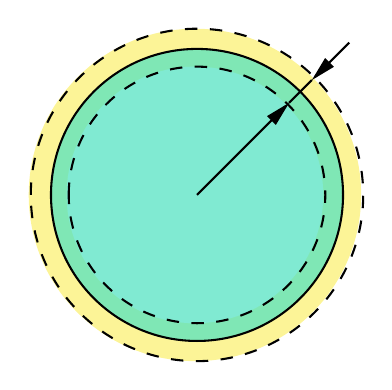
\begin{tikzpicture}[x=0.75pt,y=0.75pt,yscale=-1,xscale=1]
%uncomment if require: \path (0,300); %set diagram left start at 0, and has height of 300

%Shape: Circle [id:dp7951288433188866] 
\draw  [draw opacity=0][fill={rgb, 255:red, 248; green, 231; blue, 28 }  ,fill opacity=0.46 ][dash pattern={on 4.5pt off 4.5pt}] (111.27,180.35) .. controls (111.27,136.13) and (147.13,100.27) .. (191.35,100.27) .. controls (235.58,100.27) and (271.43,136.13) .. (271.43,180.35) .. controls (271.43,224.58) and (235.58,260.43) .. (191.35,260.43) .. controls (147.13,260.43) and (111.27,224.58) .. (111.27,180.35) -- cycle ;
%Shape: Circle [id:dp41288227165511526] 
\draw  [draw opacity=0][fill={rgb, 255:red, 255; green, 255; blue, 255 }  ,fill opacity=1 ][dash pattern={on 4.5pt off 4.5pt}] (129.54,180.35) .. controls (129.54,146.22) and (157.22,118.54) .. (191.35,118.54) .. controls (225.49,118.54) and (253.16,146.22) .. (253.16,180.35) .. controls (253.16,214.49) and (225.49,242.16) .. (191.35,242.16) .. controls (157.22,242.16) and (129.54,214.49) .. (129.54,180.35) -- cycle ;

%Shape: Circle [id:dp10315410425111105] 
\draw  [fill={rgb, 255:red, 80; green, 227; blue, 194 }  ,fill opacity=0.72 ] (122,180.35) .. controls (122,141.5) and (153.5,110) .. (192.35,110) .. controls (231.21,110) and (262.71,141.5) .. (262.71,180.35) .. controls (262.71,219.21) and (231.21,250.71) .. (192.35,250.71) .. controls (153.5,250.71) and (122,219.21) .. (122,180.35) -- cycle ;
%Straight Lines [id:da18778500428957035] 
\draw    (192.35,180.35) -- (235.29,137.41) ;
\draw [shift={(236.71,136)}, rotate = 495] [fill={rgb, 255:red, 0; green, 0; blue, 0 }  ][line width=0.08]  [draw opacity=0] (12,-3) -- (0,0) -- (12,3) -- cycle    ;
%Straight Lines [id:da5966917461276497] 
\draw    (236.71,136) -- (247.71,125) ;
%Straight Lines [id:da7760463137224431] 
\draw    (249.12,123.59) -- (265.71,107) ;
\draw [shift={(247.71,125)}, rotate = 315] [fill={rgb, 255:red, 0; green, 0; blue, 0 }  ][line width=0.08]  [draw opacity=0] (12,-3) -- (0,0) -- (12,3) -- cycle    ;
%Shape: Circle [id:dp9536544790620372] 
\draw  [dash pattern={on 4.5pt off 4.5pt}] (130.54,180.35) .. controls (130.54,146.22) and (158.22,118.54) .. (192.35,118.54) .. controls (226.49,118.54) and (254.16,146.22) .. (254.16,180.35) .. controls (254.16,214.49) and (226.49,242.16) .. (192.35,242.16) .. controls (158.22,242.16) and (130.54,214.49) .. (130.54,180.35) -- cycle ;
%Shape: Circle [id:dp8056815660877612] 
\draw  [dash pattern={on 4.5pt off 4.5pt}] (112.27,180.35) .. controls (112.27,136.13) and (148.13,100.27) .. (192.35,100.27) .. controls (236.58,100.27) and (272.43,136.13) .. (272.43,180.35) .. controls (272.43,224.58) and (236.58,260.43) .. (192.35,260.43) .. controls (148.13,260.43) and (112.27,224.58) .. (112.27,180.35) -- cycle ;




\end{tikzpicture}

    \caption{电子模式在动量空间中的分布;只有两个虚线之间的那部分电子模式被考虑}
\end{figure}

马上可以发现\eqref{eq:simple-super-conductive-hamiltonian}中$\alpha$和$\beta$其实需要是不同的,如果它们相同,由于$\vb*{k}$和$- \vb*{k}$都参与求和,根据费米子的性质,
\[
    c_{- \vb*{k} \uparrow} c_{\vb*{k} \uparrow} + c_{\vb*{k} \uparrow} c_{- \vb*{k} \uparrow} = 0,
\]
因此$\alpha = \beta$的相互作用通道实际上是不存在的。实际上,我们做了“电子能量非常低”的假设之后,这就是必然的,因为慢散射极限下只有自旋不同的电子才能够散射。(很显然,如果两个电子可以离得很近,那么它们的自旋就不能一样)
因此\eqref{eq:simple-super-conductive-hamiltonian}实际上就是
\begin{equation}
    H = \sum_{\vb*{k}} \xi_{\vb*{k}} (c^\dagger_{\vb*{k} \uparrow} c_{\vb*{k} \uparrow} + c^\dagger_{\vb*{k} \downarrow} c_{\vb*{k} \downarrow}) - V_0 \sum_{\vb*{k}, \vb*{k}'} c^\dagger_{- \vb*{k}' \downarrow} c^\dagger_{\vb*{k}' \uparrow} c_{\vb*{k} \uparrow} c_{- \vb*{k} \downarrow},
    \label{eq:superconductivity-opposite-mom}
\end{equation}
这里没有$1/2$因子,这是直接计算的结果;换一个角度,如果将$c_\uparrow$和$c_\downarrow$看成两种类型的场,则的确没有任何必要加入对称性因子。
通常我们设
\begin{equation}
    V_0 = \frac{g}{V},
\end{equation}
其中$g$是一个和系统体积无关的因子。

\eqref{eq:simple-super-conductive-hamiltonian}中有电子-电子吸引相互作用,这在\autoref{chap:conventional-metal}中从来没有出现过,那里我们处理的都是排斥相互作用,从而不必担心电子凝聚在一起,但现在有了吸引相互作用,则可能出现二电子吸在一起的束缚态。
在\eqref{eq:simple-super-conductive-hamiltonian}下,发生相互作用前两个电子必须在费米面的两端,相互作用之后两个电子还是位于费米面的两端。
这提示我们,费米面两端的两个电子可以发生配对。这就是下一节将要讨论的内容:库伯对。

在\eqref{eq:superconductivity-opposite-mom}之上还可以把被我们忽略的那些$\vb*{k} + \vb*{k}' \neq 0$的相互作用通道加回来。
本节仅讨论所谓的\concept{s波超导},所谓s波超导指的是假定有效相互作用形式就是
\begin{equation}
    H = \sum_{\vb*{k}} \xi_{\vb*{k}} (c^\dagger_{\vb*{k} \uparrow} c_{\vb*{k} \uparrow} + c^\dagger_{\vb*{k} \downarrow} c_{\vb*{k} \downarrow}) - V_0 \sum_{\vb*{k}, \vb*{k}', \vb*{q}} c^\dagger_{- \vb*{k}' \downarrow} c^\dagger_{\vb*{k}' + \vb*{q}, \uparrow} c_{\vb*{k} + \vb*{q}, \uparrow} c_{- \vb*{k} \downarrow},
    \label{eq:bcs-s-wave-full-hamiltonian}
\end{equation}
即忽略等效电子-电子耦合系数对声子动量$\vb*{q}$的依赖。
s波超导形容的是库伯对的对称性,具体它指的是什么将在\autoref{sec:su2-representation-bcs-cooper}中讨论,而\eqref{eq:bcs-s-wave-full-hamiltonian}为什么能够给出s波超导可以从它做Hubbard-Stratonovich变换之后得到的关于库伯对的有效理论的二次型部分\eqref{eq:bcs-action-delta2}中看出来。
我们这里讨论的都是单带模型,不过如果强行用$c_{\vb*{k}}$做傅里叶逆变换得到实际上只包含了一条带上的电子的“实空间场算符”$\psi(\vb*{r})$,\eqref{eq:bcs-s-wave-full-hamiltonian}对应着
\begin{equation}
    H_\text{bcs} = \frac{g}{V} \int \dd[3]{\vb*{r}} \psi_\uparrow^\dagger \psi_\downarrow^\dagger \psi_\downarrow \psi_\uparrow.
\end{equation}
这个相互作用的瞬时性来自声子本身只能持续很短时间这一事实,而它的局域性(不像库伦相互作用那样长程)则来自声子速度其实很慢这个事实。
很多教科书从上式出发引入BCS理论,而并不详细讨论其来源。

\subsection{库伯对}

\subsubsection{$SU(2)$的表示}\label{sec:su2-representation-bcs-cooper}

我们从对称性的角度出发,讨论库伯对的一般形式。
库伯对写成算符形式就是${c}^\dagger {c}^\dagger$的形式,或者等价的${c} {c}$形式。
如果其期望值不为零,那么$U(1)$对称性就破缺了,即电荷守恒对称性被破缺了(物理图像是,一部分电荷被封存到了库伯对中,不再以独立电子的形式流动)。
电荷守恒的破缺实际上是低温超导中最重要的物理,因为它意味着系统中的费米型准粒子不存在或者相较于费米液体变少了,多出来的电荷封印在库伯对中,而库伯对是可以无电阻移动的,这就导致超导现象。

库伯对序参量的一般形式是$\expval*{{c}_{\vb*{k}\alpha} {c}_{\vb*{k}' \beta}}$,或者写成实空间的形式,是$\expval*{\psi_\alpha(\vb*{r}) \psi_\beta(\vb*{r}')}$。
我们要根据没有被破缺的对称性来分析$\alpha$和$\beta$之间的关系,以及$\vb*{k}$和$\vb*{k}'$之间的关系。
可以发现\eqref{eq:simple-super-conductive-hamiltonian}具有自旋旋转不变性(这个对称性没有被破缺掉),因此相应的序参量$\expval*{{c}_{\vb*{k} \alpha} {c}_{\vb*{k}' \beta}}$应该是一个二分量的自旋协变的对象。
由于\eqref{eq:bcs-s-wave-full-hamiltonian}中忽略了自旋-轨道耦合,$\expval*{{c}_{\vb*{k}\alpha} {c}_{\vb*{k}' \beta}}$正比于一个关于$\vb*{k}$和$\vb*{k}'$的函数乘以一个关于$\alpha$和$\beta$的函数,即
\[
    \expval*{{c}_{\vb*{k} \alpha} {c}_{\vb*{k}' \beta}} \propto \Delta_\text{orbital} (\vb*{k}, \vb*{k}') \Delta_\text{spin} (\alpha, \beta).
\]

二粒子配对对应的$SU(2)$的表示为
\[
    \frac{1}{2} \otimes \frac{1}{2} = 0 \oplus 1,
\]
即可能有自旋单态也可能有自旋三重态。如果该库伯对是自旋单态,由于自旋单态只有一个基矢量
\[
    \ket{0, 0} = \frac{1}{\sqrt{2}} (\ket{\uparrow \downarrow} - \ket{\downarrow \uparrow}),
\]
将它在$\frac{1}{2} \otimes \frac{1}{2}$基底下写成矩阵形式就是$\pmqty{0 & 1 \\ -1 & 0}$,于是应该有
\[
    \expval*{{c}_{\vb*{k} \alpha} {c}_{ \vb*{k}' \beta}} \propto \epsilon_{\alpha \beta} \propto \delta_{\alpha+\beta,0},
\]
即
\begin{equation}
    \expval*{{c}_{\vb*{k} \alpha} {c}_{ \vb*{k}' \beta}} = \Delta(\vb*{k}, \vb*{k}') \epsilon_{\alpha \beta}, 
\end{equation}
其中$\epsilon$为所谓的旋量度规。
而如果该库珀对为自旋三重态,由于三重态的基底包括
\[
    \ket{1, -1} = \ket{\downarrow \downarrow}, \quad \ket{1, 0} = \frac{1}{\sqrt{2}} (\ket{\uparrow \downarrow} + \ket{\downarrow \uparrow}), \quad \ket{1, 1} = \ket{\uparrow \uparrow},
\]
我们有
\[
    [\expval*{{c}_{\vb*{k} \alpha} {c}_{ \vb*{k}' \beta}}]_{\alpha \beta} \propto c_1 \pmqty{1 & 0 \\ 0 & 0} + c_2 \pmqty{0 & 0 \\ 0 & 1} + c_3 \pmqty{0 & 1 \\ 1 & 0} ,
\]
或者也可以写成
\[
    [\expval*{{c}_{\vb*{k} \alpha} {c}_{ \vb*{k}' \beta}}]_{\alpha \beta} \propto g_1 \sigma^x \sigma^y + g_2 \sigma^y \sigma^y + g_3 \sigma^z \sigma^x,
\]
于是能够找到一个$\vb*{d}(\vb*{k}, \vb*{k}')$使得
\begin{equation}
    \expval*{{c}_{\vb*{k} \alpha} {c}_{ \vb*{k}' \beta}} = \expval*{(\vb*{d}(\vb*{k}, \vb*{k}') \cdot \vb*{\sigma}_{\alpha \beta}) \sigma^y},
\end{equation}
或者也可以直接写
\begin{equation}
    \expval*{{c}_{\vb*{k} \alpha} {c}_{ \vb*{k}' \beta}} = \vb*{d}(\vb*{k}, \vb*{k}') \cdot \vb*{\sigma}_{\alpha \beta}.
\end{equation}

\begin{back}{二体轨道波函数}{two-body-orbital-wavefunction}
    设有二体轨道波函数$\psi(\vb*{r}_1, \vb*{r}_2)$,其中$\vb*{r}_1$和$\vb*{r}_2$地位相同。
    设
    \begin{equation}
        \vb*{R} = \frac{1}{2} (\vb*{r}_1 + \vb*{r}_2), \quad \vb*{r} = \vb*{r}_1 - \vb*{r}_2.
    \end{equation}
    做傅里叶变换,有
    \[
        \begin{aligned}
            \psi(\vb*{r}_1, \vb*{r}_2) &= \frac{1}{V} \sum_{\vb*{k}_1} \sum_{\vb*{k}_2} \psi(\vb*{k}_1, \vb*{k}_2) \ee^{\ii \vb*{k}_1 \cdot \vb*{r}_1} \ee^{\ii \vb*{k}_2 \cdot \vb*{r}_2} \\
            &= \frac{1}{V} \sum_{\vb*{k}_1, \vb*{k}_2} \ee^{\ii (\vb*{k}_1 + \vb*{k}_2) \cdot \vb*{R}} \ee^{\ii (\vb*{k}_1 - \vb*{k}_2) \cdot \vb*{r} / 2} \psi(\vb*{k}_1, \vb*{k}_2).
        \end{aligned}
    \]
    这样就有
    \[
        \psi(\vb*{r}_1, \vb*{r}_2) = \frac{1}{V} \sum_{\vb*{q}} \ee^{\ii \vb*{q} \cdot \vb*{R} } \sum_{\vb*{k}'} \ee^{\ii (2 \vb*{k}' - \vb*{q}) \cdot \vb*{r} / 2} \psi(\vb*{k}', \vb*{q} - \vb*{k}'),
    \]
    或者做一个变量代换得到
    \begin{equation}
        \psi(\vb*{r}_1, \vb*{r}_2) = \frac{1}{V} \sum_{\vb*{q}} \ee^{\ii \vb*{q} \cdot \vb*{R} } \sum_{\vb*{k}} \ee^{\ii \vb*{k} \cdot \vb*{r}} \psi(\vb*{k} + \vb*{q} / 2, \vb*{q} / 2 - \vb*{k}).
    \end{equation}
    在连续空间平移不变性严格成立时,只有$\vb*{q}=0$分量,此时
    \begin{equation}
        \psi(\vb*{r}_1, \vb*{r}_2) = \frac{1}{V} \sum_{\vb*{k}} \ee^{\ii \vb*{k} \cdot (\vb*{r}_1 - \vb*{r}_2)} \psi(\vb*{k}, -\vb*{k}).
    \end{equation}
    
    可以看到交换$\vb*{r}_1$和$\vb*{r}_2$意味着将$\vb*{k}$取负号,或者说设
    \[
        \psi(\vb*{r}_1, \vb*{r}_2) = \psi'(\vb*{r}_2, \vb*{r}_1),
    \]
    则
    \[
        \psi(\vb*{k} + \vb*{q} / 2, \vb*{q} / 2 - \vb*{k}) = \psi'(- \vb*{k} + \vb*{q} / 2, \vb*{q} / 2 + \vb*{k}).
    \]

    直观地看,$\vb*{q}$是“质心动量”,而$\vb*{k}$是其中一个粒子相对质心的动量。
\end{back}

我们改用总动量$\vb*{q}$和其中一个电子相对库伯对质心的动量$\vb*{k}$标记库伯对,记作$\Delta(\vb*{k}, \vb*{q})$。
由于库伯对可以看成一个二电子波函数,它必须是反对称的(将库伯对看成一个整体,它们构成的含有多个库伯对的多体波函数是交换对称的,但是库伯对相对于组成它的电子则是交换反对称的)。
如果该库伯对是自旋单态的,那么其自旋部分是反对称的,则其轨道部分就是对称的,也即
\[
    \Delta(\vb*{k}, \vb*{q}) = \Delta(-\vb*{k}, \vb*{q}),
\]
从而固定$\vb*{q}$不变,可以将$\Delta(\vb*{k}, \vb*{q})$展开成一系列s波、d波等对称球谐函数的线性组合;
而如果该库伯对是自旋三重态的,那么其自旋部分就是对称的,于是轨道部分满足
\[
    \Delta(\vb*{k}, \vb*{q}) = -\Delta(-\vb*{k}, \vb*{q}),
\]
此时固定$\vb*{q}$不变,$\Delta(\vb*{k}, \vb*{q})$是一系列反对称球谐函数的线性组合。
容易看出单态或者三重态的出现和费米面对称性的关系,比如如果费米面不对称,那么s波配对就不能产生。

\subsubsection{库伯对作为载流子}

通常的金属中载流子都是电子和空穴。两个电子组成的玻色型准粒子库伯对携带$-2e$的电荷,是一种玻色型载流子。

电子在金属中运动时会受到晶格散射,从而有电阻。

\subsubsection{用库伯对关联函数探测s波库伯对的稳定性}

为了判断库伯对的稳定性,我们计算库伯对关联函数
\begin{equation}
    C^\text{cooper}(\vb*{q}, \ii \omega_n) = \sum_{k, k'} \expval*{\bar{c}_{-k' \downarrow} \bar{c}_{k'+q, \uparrow} c_{k+q, \uparrow} c_{-k, \downarrow}}.
\end{equation}
这里的$\beta$和$V$因子是为了让这个关联函数看起来像相互作用哈密顿量一点。
与前述寻常金属中的费曼图计算类似,为了避免发散,不能只计算有限个费曼图而必须做一定的无穷求和。
做梯形图近似
\begin{equation}
    \begin{gathered}
        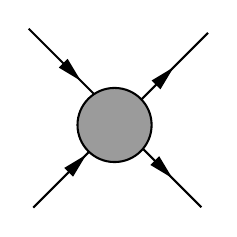
\begin{tikzpicture}[x=0.75pt,y=0.75pt,yscale=-1,xscale=1]
            %uncomment if require: \path (0,300); %set diagram left start at 0, and has height of 300
            
            %Straight Lines [id:da9345131028574916] 
            \draw    (152.5,157.2) -- (202.71,207.41) ;
            \draw [shift={(177.6,182.3)}, rotate = 225] [fill={rgb, 255:red, 0; green, 0; blue, 0 }  ][line width=0.08]  [draw opacity=0] (12,-3) -- (0,0) -- (12,3) -- cycle    ;
            %Straight Lines [id:da39542753625606863] 
            \draw    (207.71,215.2) -- (235.71,243.2) ;
            \draw [shift={(221.71,229.2)}, rotate = 225] [fill={rgb, 255:red, 0; green, 0; blue, 0 }  ][line width=0.08]  [draw opacity=0] (12,-3) -- (0,0) -- (12,3) -- cycle    ;
            %Straight Lines [id:da2774188281079233] 
            \draw    (154.71,243.41) -- (205.71,192.41) ;
            \draw [shift={(180.21,217.91)}, rotate = 495] [fill={rgb, 255:red, 0; green, 0; blue, 0 }  ][line width=0.08]  [draw opacity=0] (12,-3) -- (0,0) -- (12,3) -- cycle    ;
            %Straight Lines [id:da36864179204173797] 
            \draw    (205.71,192.41) -- (238.91,159.2) ;
            \draw [shift={(222.31,175.8)}, rotate = 495] [fill={rgb, 255:red, 0; green, 0; blue, 0 }  ][line width=0.08]  [draw opacity=0] (12,-3) -- (0,0) -- (12,3) -- cycle    ;
            %Shape: Circle [id:dp41808205207920834] 
            \draw  [fill={rgb, 255:red, 155; green, 155; blue, 155 }  ,fill opacity=1 ] (176,203.59) .. controls (176,193.73) and (183.99,185.73) .. (193.85,185.73) .. controls (203.71,185.73) and (211.71,193.73) .. (211.71,203.59) .. controls (211.71,213.45) and (203.71,221.44) .. (193.85,221.44) .. controls (183.99,221.44) and (176,213.45) .. (176,203.59) -- cycle ;
            \end{tikzpicture}                
    \end{gathered} = \begin{gathered}
        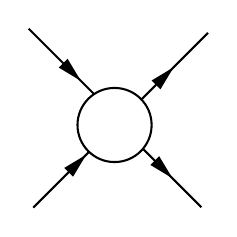
\begin{tikzpicture}[x=0.75pt,y=0.75pt,yscale=-1,xscale=1]
            %uncomment if require: \path (0,300); %set diagram left start at 0, and has height of 300
            
            %Straight Lines [id:da9345131028574916] 
            \draw    (152.5,157.2) -- (202.71,207.41) ;
            \draw [shift={(177.6,182.3)}, rotate = 225] [fill={rgb, 255:red, 0; green, 0; blue, 0 }  ][line width=0.08]  [draw opacity=0] (12,-3) -- (0,0) -- (12,3) -- cycle    ;
            %Straight Lines [id:da39542753625606863] 
            \draw    (207.71,215.2) -- (235.71,243.2) ;
            \draw [shift={(221.71,229.2)}, rotate = 225] [fill={rgb, 255:red, 0; green, 0; blue, 0 }  ][line width=0.08]  [draw opacity=0] (12,-3) -- (0,0) -- (12,3) -- cycle    ;
            %Straight Lines [id:da2774188281079233] 
            \draw    (154.71,243.41) -- (205.71,192.41) ;
            \draw [shift={(180.21,217.91)}, rotate = 495] [fill={rgb, 255:red, 0; green, 0; blue, 0 }  ][line width=0.08]  [draw opacity=0] (12,-3) -- (0,0) -- (12,3) -- cycle    ;
            %Straight Lines [id:da36864179204173797] 
            \draw    (205.71,192.41) -- (238.91,159.2) ;
            \draw [shift={(222.31,175.8)}, rotate = 495] [fill={rgb, 255:red, 0; green, 0; blue, 0 }  ][line width=0.08]  [draw opacity=0] (12,-3) -- (0,0) -- (12,3) -- cycle    ;
            %Shape: Circle [id:dp41808205207920834] 
            \draw  [fill={rgb, 255:red, 255; green, 255; blue, 255 }  ,fill opacity=1 ] (176,203.59) .. controls (176,193.73) and (183.99,185.73) .. (193.85,185.73) .. controls (203.71,185.73) and (211.71,193.73) .. (211.71,203.59) .. controls (211.71,213.45) and (203.71,221.44) .. (193.85,221.44) .. controls (183.99,221.44) and (176,213.45) .. (176,203.59) -- cycle ;
            \end{tikzpicture}                    
    \end{gathered} + \begin{gathered}
        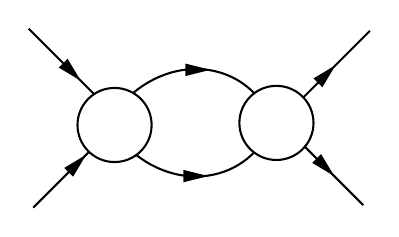
\begin{tikzpicture}[x=0.75pt,y=0.75pt,yscale=-1,xscale=1]
            %uncomment if require: \path (0,300); %set diagram left start at 0, and has height of 300
            
            %Curve Lines [id:da0323321140047681] 
            \draw    (165.71,161.41) .. controls (188.71,190.79) and (225.71,187.79) .. (239.71,161.79) ;
            %Straight Lines [id:da23429070529223384] 
            \draw    (211,182.2) ;
            \draw [shift={(211,182.2)}, rotate = 180] [fill={rgb, 255:red, 0; green, 0; blue, 0 }  ][line width=0.08]  [draw opacity=0] (12,-3) -- (0,0) -- (12,3) -- cycle    ;
            %Curve Lines [id:da006405555941071395] 
            \draw    (165.71,151.59) .. controls (188.71,122.21) and (225.71,125.21) .. (239.71,151.21) ;
            %Straight Lines [id:da7859806184703646] 
            \draw    (124.5,111.2) -- (174.71,161.41) ;
            \draw [shift={(149.6,136.3)}, rotate = 225] [fill={rgb, 255:red, 0; green, 0; blue, 0 }  ][line width=0.08]  [draw opacity=0] (12,-3) -- (0,0) -- (12,3) -- cycle    ;
            %Straight Lines [id:da979040764755357] 
            \draw    (126.71,197.41) -- (177.71,146.41) ;
            \draw [shift={(152.21,171.91)}, rotate = 495] [fill={rgb, 255:red, 0; green, 0; blue, 0 }  ][line width=0.08]  [draw opacity=0] (12,-3) -- (0,0) -- (12,3) -- cycle    ;
            %Shape: Circle [id:dp6186819574350089] 
            \draw  [fill={rgb, 255:red, 255; green, 255; blue, 255 }  ,fill opacity=1 ] (148,157.59) .. controls (148,147.73) and (155.99,139.73) .. (165.85,139.73) .. controls (175.71,139.73) and (183.71,147.73) .. (183.71,157.59) .. controls (183.71,167.45) and (175.71,175.44) .. (165.85,175.44) .. controls (155.99,175.44) and (148,167.45) .. (148,157.59) -- cycle ;
            %Straight Lines [id:da26833664483472486] 
            \draw    (257.71,168.2) -- (285.71,196.2) ;
            \draw [shift={(271.71,182.2)}, rotate = 225] [fill={rgb, 255:red, 0; green, 0; blue, 0 }  ][line width=0.08]  [draw opacity=0] (12,-3) -- (0,0) -- (12,3) -- cycle    ;
            %Straight Lines [id:da4482068470519842] 
            \draw    (255.71,145.41) -- (288.91,112.2) ;
            \draw [shift={(272.31,128.8)}, rotate = 495] [fill={rgb, 255:red, 0; green, 0; blue, 0 }  ][line width=0.08]  [draw opacity=0] (12,-3) -- (0,0) -- (12,3) -- cycle    ;
            %Shape: Circle [id:dp8625776854304812] 
            \draw  [fill={rgb, 255:red, 255; green, 255; blue, 255 }  ,fill opacity=1 ] (226,156.59) .. controls (226,146.73) and (233.99,138.73) .. (243.85,138.73) .. controls (253.71,138.73) and (261.71,146.73) .. (261.71,156.59) .. controls (261.71,166.45) and (253.71,174.44) .. (243.85,174.44) .. controls (233.99,174.44) and (226,166.45) .. (226,156.59) -- cycle ;
            %Straight Lines [id:da5905789317550543] 
            \draw    (212,131) ;
            \draw [shift={(212,131)}, rotate = 180] [fill={rgb, 255:red, 0; green, 0; blue, 0 }  ][line width=0.08]  [draw opacity=0] (12,-3) -- (0,0) -- (12,3) -- cycle    ;
            \end{tikzpicture}            
    \end{gathered} + \cdots,
\end{equation}
能够计算得到顶角函数
\begin{equation}
    \Gamma_q = - \frac{g}{1 - \frac{g}{\beta V} \sum_{p} G^0_{p+q} G^0_{-p}} ,
    \label{eq:bcs-four-e-vertex-eff}
\end{equation}
从而
\begin{equation}
    C^\text{cooper}(\vb*{q}, \ii \omega_n) = \sum_{k, k'} \expval*{\bar{c}_{-k' \downarrow} \bar{c}_{k'+q, \uparrow} c_{k+q, \uparrow} c_{-k, \downarrow}}_0 + \frac{g}{1 - \frac{g}{\beta V} \sum_{p} G^0_{p+q} G^0_{-p}}.
    \label{eq:bcs-cooper-pair-correlation}
\end{equation}
上式的第一项可以通过Wick定理,按照\autoref{sec:rpa-semi-classical-dynamical}的方法可以计算出来。
第二项计算如下。我们有
\[
    - \frac{1}{\beta V} \sum_p G^0_{p+q} G^0_{-p} = - \frac{1}{\beta V} \sum_{p^0, \vb*{p}} \frac{1}{\ii (p^0 + q^0) - \xi_{\vb*{p} + \vb*{q}}} \frac{1}{- \ii p^0 - \xi_{\vb*{p}}},
\]
这里用到了$\xi_{\vb*{p}}$和$\xi_{-\vb*{p}}$一样这一事实。
同样使用\autoref{sec:rpa-semi-classical-dynamical}中使用过的方法,根据
\[
    \frac{1}{\beta} \sum_{\ii \omega_n} F(\ii \omega_n) = - \frac{1}{2\pi \ii} \oint \dd{z} F(z) f(z),
\]
我们有
\[
    \begin{aligned}
        - \frac{1}{\beta V} \sum_{p^0, \vb*{p}} \frac{1}{\ii (p^0 + q^0) - \xi_{\vb*{p} + \vb*{q}}} \frac{1}{- \ii p^0 - \xi_{\vb*{p}}} &= - \sum_{\vb*{p}} \frac{1}{V} \frac{1}{2\pi \ii} \oint \dd{z} f(z) \frac{1}{z + \ii q^0 - \xi_{\vb*{p}+\vb*{q}}} \frac{1}{z+\xi_{\vb*{p}}} \\
        &= \frac{1}{V} \sum_{\vb*{p}} \left( \frac{f(-\xi_{\vb*{p}})}{- \xi_{\vb*{p}} + \ii q^0 - \xi_{\vb*{p}+\vb*{q}}} + \frac{f(\xi_{\vb*{p}+\vb*{q}} - \ii q^0)}{\xi_{\vb*{p}+\vb*{q}} - \ii q^0 + \xi_{\vb*{p}}} \right) \\
        &= \frac{1}{V} \sum_{\vb*{p}} \frac{1 - f(\xi_{\vb*{p}}) - f(\xi_{\vb*{p}+\vb*{q}})}{\ii q^0 - \xi_{\vb*{p}} - \xi_{\vb*{p} + \vb*{q}}},
    \end{aligned}
\]
即
\begin{equation}
    G^\text{cooper}(q) - C^\text{cooper}_0(q) = \frac{1}{1 - \frac{g}{V} \sum_{\vb*{p}} \frac{f(\xi_{\vb*{p}}) + f(\xi_{\vb*{p}+\vb*{q}}) - 1}{\ii q^0 - \xi_{\vb*{p}} - \xi_{\vb*{p} + \vb*{q}}}}.
    \label{eq:bcs-cooper-pair-correlation-strange-part}
\end{equation}

上式右边的奇异性实际上有温度依赖。考虑$q=0$的情况,此时
\[
    \frac{g}{V} \sum_{\vb*{p}} \frac{f(\xi_{\vb*{p}}) + f(\xi_{\vb*{p}+\vb*{q}}) - 1}{\ii q^0 - \xi_{\vb*{p}} - \xi_{\vb*{p} + \vb*{q}}} = g \int \dd{\epsilon} D(\epsilon) \frac{1 - 2f(\epsilon)}{2\epsilon}.
\]
这里有几个截断。首先根据\eqref{eq:bcs-small-sphere-around-fermi-surface},$\epsilon$的上下限为$\pm \omega_\text{D} / 2$,且$1-2f(\epsilon)$在$\epsilon > 0$和$\epsilon < 0$时差一个正负号,因此
\[
    \begin{aligned}
        g \int \dd{\epsilon} D(\epsilon) \frac{1 - 2f(\epsilon)}{2\epsilon} &= g \int_{-\omega_\text{D}/2}^{\omega_\text{D}/2} \dd{\epsilon} D(\epsilon) \frac{1 - 2f(\epsilon)}{2\epsilon} \\
        &= g \int_{0}^{\omega_\text{D}/2} \dd{\epsilon} D(\epsilon) \frac{1 - 2f(\epsilon)}{\epsilon}.
    \end{aligned}
\]
其次,$f(\epsilon)$只有在$\epsilon$和$0$不那么接近时才有明显的非零值,在$\epsilon \to 0^+$时$f(\epsilon)$快速衰减,因此我们需要做一个大小大体上正比于$T$的红外截断,即
\[
    g \int_{0}^{\omega_\text{D}/2} \dd{\epsilon} D(\epsilon) \frac{1 - 2f(\epsilon)}{\epsilon} \sim g D(0) \int_{T}^{\omega_\text{D}/2} \dd{\epsilon} \frac{1}{\epsilon} \sim g D(0) \ln\frac{\omega_\text{D}}{T},
\]
从而\eqref{eq:bcs-cooper-pair-correlation-strange-part}右边的分母在
\[
    1 \sim g D(0) \ln\frac{\omega_\text{D}}{T},
\]
即
\begin{equation}
    T \to T_\text{c} \sim \omega_\text{D} \exp(- \frac{1}{g D(0)})
\end{equation}
时变为零,关联函数发散。以上数量级估计中的近似之处在于$T$前面可以乘以一个常数,除此以外没有什么近似,因此
\begin{equation}
    T_\text{c} = \const \times \omega_\text{D} \exp(- \frac{1}{g D(0)})
\end{equation}
前面的常数只要正确,就是足够精确的。关联函数的发散大体上是
\[
    \frac{1}{1 - g D(0) \ln \frac{\omega_\text{D}}{T}} \sim - \frac{T_\text{c}}{g D(0) (T - T_\text{c})}.
\]

以上推导暗示两件事:首先,在$T < T_\text{c}$时仅仅做梯形图近似是不够的,即,如果以费米海为基态,那么需要纳入考虑的量子涨落非常大,这暗示,此时我们其实\emph{不应该}以费米海为基态,即费米面出现了不稳定性,一个对称性自发破缺发生了;且做梯形图近似会出现发散这件事实际上还暗示了对称性自发破缺的序参量,这点我们在\eqref{eq:bcs-cooper-2nd-propagator}前后的讨论中会提到。
其次,$q=0$时$T \to T_\text{c}$时关联函数出现极点,这是相变点附近的典型行为,即$T = T_\text{c}$处可能存在相变。

在远离$T = T_\text{c}, q = 0$点处,关联函数\eqref{eq:bcs-cooper-pair-correlation}显然有有限大虚部
以上几个暗示放在一起,似乎说明,在低温下系统会发生对称性自发破缺,库伯对是稳定的,而且系统基态可能就是由大量库伯对构成的。

\subsection{s波BCS超导的平均场研究}

\subsubsection{平均场序参量哈密顿量}

\begin{back}{用平均场近似研究对称性自发破缺}{mean-field-method-symmetry-broken}
    在\autoref{back:scf-method}中我们引入了平均场方法,很容易看出,平均场方法可以用于处理对称性自发破缺问题。
    我们只需要写下一个在被破缺的那部分对称性存在时一定为零的格林函数,然后用平均场近似计算它就可以,如果在一些条件下它不为零,那么就可能发生了对称性自发破缺。
    这个格林函数出于显然的原因,被称为“平均场序参量”。需要注意,在以费米海为基态的费曼规则中看起来不太对头的那些格林函数(如$\expval{c c}$,画成图是两个相对的箭头,根据$U(1)$对称性为零)也可以做平均场序参量,因为无法保证对称性自发破缺后这些格林函数真的还是零。

    单纯地使用有限阶微扰论不足以研究对称性自发破缺,因为对称性自发破缺会让基态发生变化,在假的基态附近做微扰是无法给出可靠的结果的。
    平均场方法则将无数个费曼图重求和了,实际上是一种非微扰方法,因此可以捕捉到对称性自发破缺。
    然而平均场方法认为存在对称性自发破缺的情况下未必真的有对称性自发破缺,因为平均场方法忽略了许多其它的图,倾向于低估量子涨落。
    即使平均场方法预言的对称性自发破缺是真实的,它给出的相变点位置通常也不可靠,因此只能作为定性方法使用。
    另一个平均场方法不可靠的地方是,平均场方法假定序参量$\expval{cc}$是没有任何涨落的,系统中仅有的涨落是费米场,而这当然不是事实:序参量本身是可以涨落的,而且这些涨落是系统的低能激发的重要成分。

    最后应当指出,其实平均场近似不仅仅适用于费米子系统,它对各种自由度的模型都是适用的。
\end{back}

平均场近似忽略了库伯对的涨落,即我们假定库伯对总是在它们的基态上。此时由于空间平移对称性没有破缺,\autoref{back:two-body-orbital-wavefunction}中的$\vb*{q} = 0$,即我们可以认为
\[
    \expval*{{c}_{\vb*{k}\alpha} {c}_{\vb*{k}' \beta}} \propto \delta(\vb*{k} + \vb*{k}').
\]
换而言之,我们只考虑总动量为零的配对$\expval*{{c}_{\vb*{k} \alpha} {c}_{- \vb*{k} \beta}}$。
这个做法的合理性也可以通过注意到最重要的相互作用通道是\eqref{eq:superconductivity-opposite-mom}来得到辩护——实际上这样做更加合理,因为在存在电子凝聚时一般很难判断空间平移对称性是不是真的没被破缺,例如我们在\autoref{sec:spin-spin-nn-interaction-sdw}中就能够看到一个空间平移对称性破缺的例子。

对\eqref{eq:simple-super-conductive-hamiltonian}做平均场近似,有
\[
    \begin{aligned}
        & \quad {c}^\dagger_{(\vb*{k} + \vb*{q}) \alpha} {c}^\dagger_{( - \vb*{k} - \vb*{q}) \beta} {c}_{-\vb*{k} \beta} {c}_{\vb*{k} \alpha} \\
        &\approx \expval*{{c}^\dagger_{(\vb*{k} + \vb*{q}) \alpha} {c}^\dagger_{( - \vb*{k} - \vb*{q}) \beta}} {c}_{-\vb*{k} \beta} {c}_{\vb*{k} \alpha} + {c}^\dagger_{(\vb*{k} + \vb*{q}) \alpha} {c}^\dagger_{( - \vb*{k} - \vb*{q}) \beta} \expval*{{c}_{-\vb*{k} \beta} {c}_{\vb*{k} \alpha}} - \expval*{{c}^\dagger_{(\vb*{k} + \vb*{q}) \alpha} {c}^\dagger_{( - \vb*{k} - \vb*{q}) \beta} {c}_{-\vb*{k} \beta} {c}_{\vb*{k} \alpha}},
    \end{aligned}
\]
重新选定求和哑指标,并略去对体系动力学没有影响的常数项,得到
\begin{equation}
    {H}_\text{MF} = \sum_{\vb*{k}, \alpha} (\epsilon_{\vb*{k}} - \mu) {c}_{\vb*{k} \alpha}^\dagger {c}_{\vb*{k} \alpha} - \frac{V_0}{2} \sum_{\vb*{k}, \vb*{k}', \alpha, \beta} \left(
        \expval*{{c}_{-\vb*{k} \beta} {c}_{\vb*{k} \alpha}} {c}^\dagger_{\vb*{k}' \alpha} {c}^\dagger_{- \vb*{k}' \beta} + \text{h.c.} 
    \right).
    \label{eq:superconductivity-mf-original}
\end{equation}
的确,电荷守恒对称性被破缺了,原因是电子形成库伯对之后看起来就像被“冻结”了一样,因此不再被计入${c}^\dagger$自由度中,而是被计入序参量$\expval*{{c}_{-\vb*{k} \beta} {c}_{\vb*{k} \alpha}}$中。

现在我们考虑单态、s波的库伯对,这样发生配对的就是一个$\vb*{k}, \uparrow$态的电子和一个$-\vb*{k}, \downarrow$态的电子,或者做一个自旋旋转。总之,序参量可以选取为
\begin{equation}
    \Delta = - \frac{V_0}{2} \sum_{\vb*{k}} (
        \expval*{{c}_{-\vb*{k}\uparrow} {c}_{\vb*{k} \downarrow}} - \expval*{{c}_{-\vb*{k} \downarrow} {c}_{\vb*{k} \uparrow}}
    ) = -V_0 \sum_{\vb*{k}} \expval*{{c}_{-\vb*{k}\uparrow} {c}_{\vb*{k} \downarrow}} ,
    \label{eq:superconductive-order-parameter}
\end{equation}
则\eqref{eq:superconductivity-mf-original}中只有尖括号内满足$\alpha = -\beta$的项才能够保留下来,计算得到
\begin{equation}
    {H}_\text{MF} = \sum_{\vb*{k}, \alpha} \xi_{\vb*{k}} {c}_{\vb*{k} \alpha}^\dagger {c}_{\vb*{k} \alpha} 
    + \Delta \sum_{\vb*{k}} {c}_{-\vb*{k} \downarrow}^\dagger {c}^\dagger_{\vb*{k} \uparrow}
    + \Delta^* \sum_{\vb*{k}} {c}_{\vb*{k} \uparrow} {c}_{-\vb*{k} \downarrow}.
    \label{eq:s-wave-superconductive-hamiltonian}
\end{equation}

\subsubsection{平均场近似下的系统的费米型激发}

下面我们用一个幺正变换重新定义一组准粒子(这就称为\concept{Bogoliubov变换}),使这组准粒子本身是费米子,并且能够让\eqref{eq:s-wave-superconductive-hamiltonian}对角化(从而这组准粒子的能谱就是\eqref{eq:s-wave-energy-band})。
设这组Bogoliubov准粒子为$\gamma^\dagger_{\vb*{k} \alpha}$,我们要求费米子的对易关系
\begin{equation}
    \acomm*{{\gamma}_{\vb*{k}_1 \alpha}}{{\gamma}^\dagger_{\vb*{k}_2 \beta}} = \delta_{\vb*{k}_1 \vb*{k}_2} \delta_{\alpha \beta}, \quad \acomm*{{\gamma}_{\vb*{k}_1 \alpha}}{{\gamma}_{\vb*{k}_2 \beta}} = 0
\end{equation}
成立。可以看到,以下正交变换
\begin{equation}
    \pmqty{{\gamma}_{\vb*{k} \uparrow} \\ {\gamma}^\dagger_{-\vb*{k} \downarrow}} = \pmqty{u_{\vb*{k}} & -v_{\vb*{k}} \\ v_{\vb*{k}} & u_{\vb*{k}}} \pmqty{{c}_{\vb*{k} \uparrow} \\ {c}^\dagger_{-\vb*{k} \downarrow}},
    \quad u_{\vb*{k}}^2 + v_{\vb*{k}}^2 = 1
\end{equation}
能够给出正确的对易关系。于是我们将\eqref{eq:s-wave-superconductive-hamiltonian}改写成
\begin{equation}
    H_\text{MF} = \sum_{\vb*{k}} \pmqty{c^\dagger_{\vb*{k} \uparrow} & c_{- \vb*{k} \downarrow}} \pmqty{ \xi_{\vb*{k}} & - \Delta \\ - \Delta^* & - \xi_{\vb*{k}} } \pmqty{c_{\vb*{k} \uparrow} \\ c^\dagger_{- \vb*{k} \downarrow}}.
    \label{eq:superconductivity-mf-matrix}
\end{equation}
将其中的矩阵分解成$U^\dagger \diag(E_1, E_2) U$的形式,其中$U$是正交矩阵,就能够得到Bogoliubov准粒子。%
\footnote{从电子到Bogoliubov准粒子的变换未必是正交变换,有时候真的要用一个非正交变换;关键在于对易关系必须正确,不是所有的线性变换形式都能够给出正确的对易关系。}%

然而\eqref{eq:superconductivity-mf-matrix}中的矩阵做特征分解得到的$U$是否是正交矩阵是存疑的。
我们能够确定$U$是幺正的,但是是否有$u_{\vb*{k}}^2 + v_{\vb*{k}}^2 = 1$成立呢?
我们做一个大胆的假设,假定$\Delta$为实数。
实际情况如何,需要通过系统地分析序参量的场论和对称性自发破缺之后的基态和其上的涨落才能够得到,我们将在\autoref{sec:superconductivity-gl}中验证这一点。
这里我们姑且假定$\Delta$为实数,计算所有能够计算的东西,如果一切都符合得很好,那么这个假设是有道理的。
$\Delta$为实数时\eqref{eq:superconductivity-mf-matrix}中的矩阵是实对称矩阵,一定能够做特征分解,且特征向量是实的,彼此正交。
此时计算本征值得到
\begin{equation}
    E_{\vb*{k}} = \pm \sqrt{ \xi_{\vb*{k}}^2 + \abs{\Delta}^2 }.
    \label{eq:s-wave-energy-band}
\end{equation}
取$E_{\vb*{k}}$为正值,特征分解得到
\[
    \pmqty{ \xi_{\vb*{k}} & - \Delta \\ - \Delta & - \xi_{\vb*{k}} } = \pmqty{u_{\vb*{k}} & v_{\vb*{k}} \\ - v_{\vb*{k}} & u_{\vb*{k}}} \pmqty{\dmat{E_{\vb*{k}}, - E_{\vb*{k}}}} \pmqty{u_{\vb*{k}} & -v_{\vb*{k}} \\ v_{\vb*{k}} & u_{\vb*{k}}},
\]
其中
\begin{equation}
    u_{\vb*{k}} = \sqrt{\frac{E_{\vb*{k}} + \xi_{\vb*{k}}}{2 E_{\vb*{k}}}}, \quad v_{\vb*{k}} = \sqrt{\frac{E_{\vb*{k}} - \xi_{\vb*{k}}}{2 E_{\vb*{k}}}}.
\end{equation}
这就得到了Bogoliubov变换的显式形式:
\begin{equation}
    \begin{cases}
        {\gamma}_{\vb*{k} \uparrow} = u_{\vb*{k}} {c}_{\vb*{k} \uparrow} - v_{\vb*{k}} {c}_{-\vb*{k} \downarrow}^\dagger, \\
        {\gamma}_{\vb*{k} \downarrow} = u_{\vb*{k}} {c}_{\vb*{k} \downarrow} + v_{\vb*{k}} {c}_{-\vb*{k} \uparrow}^\dagger,
    \end{cases}
    \label{eq:bogoliubov-transform}
\end{equation}
$\gamma_{\vb*{k} \uparrow}^\dagger$粒子的能量是$E_{\vb*{k}}$,$\gamma_{\vb*{k} \downarrow}^\dagger$粒子的能量是$- E_{\vb*{k}}$。
逆变换为
\begin{equation}
    \begin{cases}
        {c}_{\vb*{k} \uparrow} = u_{\vb*{k}} {\gamma}_{\vb*{k} \uparrow} + v_{\vb*{k}} {\gamma}_{-\vb*{k} \downarrow}^\dagger, \\
        {c}_{\vb*{k} \downarrow} = u_{\vb*{k}} {\gamma}_{\vb*{k} \downarrow} - v_{\vb*{k}} {\gamma}_{-\vb*{k} \uparrow}^\dagger.
    \end{cases}
    \label{eq:inverse-bogoliubov-transform}
\end{equation}

\begin{figure}
    \centering
    \subfigure[蓝色曲线是未配对电子的能谱,同时包含两种自旋;红色曲线是将一种电子当成空穴以后的能谱]{
        

\tikzset{every picture/.style={line width=0.75pt}} %set default line width to 0.75pt        

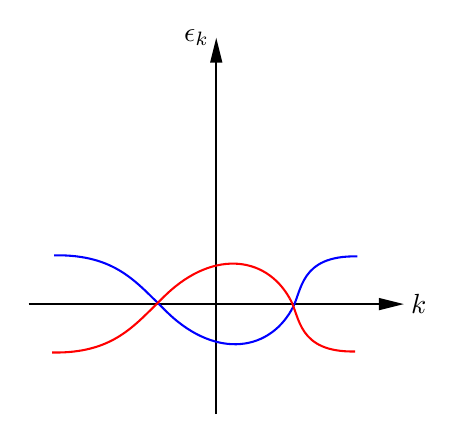
\begin{tikzpicture}[x=0.75pt,y=0.75pt,yscale=-1,xscale=1]
%uncomment if require: \path (0,300); %set diagram left start at 0, and has height of 300

%Straight Lines [id:da8505610866933] 
\draw    (101,219) -- (279.71,219) ;
\draw [shift={(281.71,219)}, rotate = 180] [fill={rgb, 255:red, 0; green, 0; blue, 0 }  ][line width=0.08]  [draw opacity=0] (12,-3) -- (0,0) -- (12,3) -- cycle    ;
%Straight Lines [id:da8248225909624645] 
\draw    (191.35,272) -- (191.35,92.69) ;
\draw [shift={(191.35,90.69)}, rotate = 450] [fill={rgb, 255:red, 0; green, 0; blue, 0 }  ][line width=0.08]  [draw opacity=0] (12,-3) -- (0,0) -- (12,3) -- cycle    ;
%Curve Lines [id:da9081456724098811] 
\draw [color={rgb, 255:red, 0; green, 0; blue, 255 }  ,draw opacity=1 ]   (166.29,221.5) .. controls (189.07,244.89) and (215.79,243) .. (227.79,221.5) ;
%Curve Lines [id:da5382231783747533] 
\draw [color={rgb, 255:red, 0; green, 0; blue, 255 }  ,draw opacity=1 ]   (113.29,195.5) .. controls (142.79,195) and (152.79,208.5) .. (166.29,221.5) ;
%Curve Lines [id:da8190264329883021] 
\draw [color={rgb, 255:red, 0; green, 0; blue, 255 }  ,draw opacity=1 ]   (259.29,196) .. controls (231.29,195.5) and (232.79,213) .. (227.79,221.5) ;

%Curve Lines [id:da487854281259237] 
\draw [color={rgb, 255:red, 255; green, 0; blue, 0 }  ,draw opacity=1 ]   (165.29,216.33) .. controls (188.07,192.94) and (214.79,194.83) .. (226.79,216.33) ;
%Curve Lines [id:da8067779262113395] 
\draw [color={rgb, 255:red, 255; green, 0; blue, 0 }  ,draw opacity=1 ]   (112.29,242.33) .. controls (141.79,242.83) and (151.79,229.33) .. (165.29,216.33) ;
%Curve Lines [id:da43392835439828703] 
\draw [color={rgb, 255:red, 255; green, 0; blue, 0 }  ,draw opacity=1 ]   (258.29,241.83) .. controls (230.29,242.33) and (231.79,224.83) .. (226.79,216.33) ;


% Text Node
\draw (283.71,219) node [anchor=west] [inner sep=0.75pt]    {$\boldsymbol{k}$};
% Text Node
\draw (189.35,90.69) node [anchor=east] [inner sep=0.75pt]    {$\epsilon _{\boldsymbol{k}}$};


\end{tikzpicture}

    }
    \subfigure[Bogoliubov准粒子的能谱,相当于是将一种自旋的电子视为电子,一种自旋的电子视为空穴,然后打开能隙]{
        

\tikzset{every picture/.style={line width=0.75pt}} %set default line width to 0.75pt        

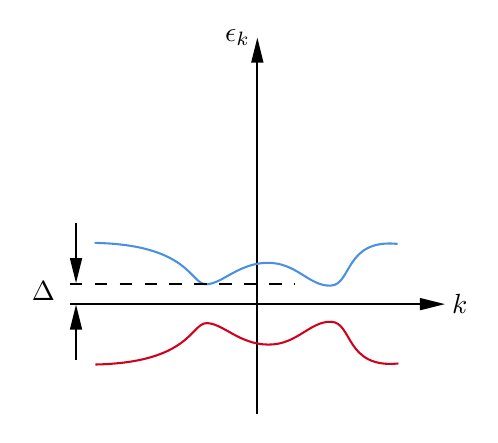
\begin{tikzpicture}[x=0.75pt,y=0.75pt,yscale=-1,xscale=1]
%uncomment if require: \path (0,300); %set diagram left start at 0, and has height of 300

%Straight Lines [id:da3923768503429792] 
\draw    (93,198) -- (271.71,198) ;
\draw [shift={(273.71,198)}, rotate = 180] [fill={rgb, 255:red, 0; green, 0; blue, 0 }  ][line width=0.08]  [draw opacity=0] (12,-3) -- (0,0) -- (12,3) -- cycle    ;
%Straight Lines [id:da007460559717310078] 
\draw    (183.35,251) -- (183.35,71.69) ;
\draw [shift={(183.35,69.69)}, rotate = 450] [fill={rgb, 255:red, 0; green, 0; blue, 0 }  ][line width=0.08]  [draw opacity=0] (12,-3) -- (0,0) -- (12,3) -- cycle    ;
%Curve Lines [id:da5016211924753684] 
\draw [color={rgb, 255:red, 74; green, 144; blue, 226 }  ,draw opacity=1 ]   (104.95,168.5) .. controls (150.96,169.43) and (150.96,188.43) .. (158.63,188.43) .. controls (166.3,188.43) and (174.27,178.19) .. (188.3,178.1) .. controls (202.32,178.01) and (208.3,189.43) .. (218.63,189.1) .. controls (228.96,188.77) and (225.3,166.43) .. (250.95,169) ;
%Curve Lines [id:da07180929244633205] 
\draw [color={rgb, 255:red, 208; green, 2; blue, 27 }  ,draw opacity=1 ]   (105.29,227.11) .. controls (151.3,226.17) and (151.3,207.17) .. (158.96,207.17) .. controls (166.63,207.17) and (174.61,217.42) .. (188.63,217.51) .. controls (202.65,217.6) and (208.63,206.17) .. (218.96,206.51) .. controls (229.3,206.84) and (225.63,229.17) .. (251.29,226.61) ;
%Straight Lines [id:da7044155195594983] 
\draw  [dash pattern={on 4.5pt off 4.5pt}]  (93,188.32) -- (201.49,188.32) ;
%Straight Lines [id:da29258181497582525] 
\draw    (96,159.04) -- (96,185.84) ;
\draw [shift={(96,187.84)}, rotate = 270] [fill={rgb, 255:red, 0; green, 0; blue, 0 }  ][line width=0.08]  [draw opacity=0] (12,-3) -- (0,0) -- (12,3) -- cycle    ;
%Straight Lines [id:da5558233224671132] 
\draw    (96,200.27) -- (96,225.04) ;
\draw [shift={(96,198.27)}, rotate = 90] [fill={rgb, 255:red, 0; green, 0; blue, 0 }  ][line width=0.08]  [draw opacity=0] (12,-3) -- (0,0) -- (12,3) -- cycle    ;

% Text Node
\draw (275.71,198) node [anchor=west] [inner sep=0.75pt]    {$\boldsymbol{k}$};
% Text Node
\draw (181.35,69.69) node [anchor=east] [inner sep=0.75pt]    {$\epsilon _{\boldsymbol{k}}$};
% Text Node
\draw (73.2,185.52) node [anchor=north west][inner sep=0.75pt]    {$\Delta $};


\end{tikzpicture}

    }
    \caption{Bogoliubov准粒子的能谱}
    \label{fig:superconductivity-bogoliubov}
\end{figure}

这个结果具有粒子-空穴对称性,但是这并不具有太多物理意义,因为它实际上是对角化时交换了一对产生湮灭算符,从而把一部分粒子自由度写成了空穴而已。

没有$\Delta$时只考虑轨道波函数的话有一条能带,就是$E = \xi_{\vb*{k}}$,考虑有一上一下两种自旋那就有两条能带。
对金属$\xi_{\vb*{k}}$是无能隙的,即$\xi_{\vb*{k}}$存在零点。%
\eqref{eq:s-wave-energy-band}中,序参量$\Delta$的存在让我们得到了两条彼此存在能隙的能带。
由费米分布,$E = - E_{\vb*{k}}$那一条带,即$\gamma_{\vb*{k} \downarrow}$那一条带完全被占据(我们已经将化学势算在$\xi_{\vb*{k}}$中了,无需重复考虑化学势)。
因此基态附近的费米型激发就是$\gamma_{\vb*{k} \uparrow}$准粒子和$\gamma_{\vb*{k} \downarrow}$准空穴,它们的能谱都是$E = E_{\vb*{k}}$,并且有一个大小为$\Delta$的能隙。(见\autoref{fig:superconductivity-bogoliubov})

系统的费米型激发存在能隙这件事是值得注意的。我们这里以$\xi_{\vb*{k}}$为电子能量,即已经扣除了化学势,如果系统是普通意义上的导体,那么不应该有能隙,因为化学势在某一条能带内部,费米面附近的电子可以被任意小的能量激发。
但是\eqref{eq:simple-super-conductive-hamiltonian}的费米型激发是有能隙的,这意味着在零温处根本不存在普通的能带电子,所有的电子都被“封印”在库伯对里面了,并且小的扰动只会让库伯对“海”发生小的扭曲,不会让费米型激发出现,因为费米型激发是有能隙的。
此时也不存在费米面,因为有费米面则费米面附近的费米型载流子是无能隙的,而这并非这里的情况。
略微考虑一下我们就会发现,${\Delta}$正是拆开一个库伯对,从中释放出电子需要的能量,可以说就是库伯对的结合能,系统的费米型激发有能隙即$\Delta \neq 0$意味着库伯对是稳定的,不会被任意小的扰动拆散。

% TODO:系统基态:Bogoliubov准粒子真空态

\subsubsection{平均场自洽计算}

得到平均场理论后我们来做自洽计算。将\eqref{eq:inverse-bogoliubov-transform}代入\eqref{eq:superconductive-order-parameter},并利用近独立电子气的数目
\[
    \expval*{{\gamma}_{\vb*{k} \alpha}^\dagger {\gamma}_{\vb*{k} \alpha}} = f(E_{\vb*{k}}) =  \frac{1}{\ee^{\beta E_{\vb*{k}}} + 1},
\]
得到
\[
    \Delta = - V_0 \sum_{\vb*{k}} u_{\vb*{k}} v_{\vb*{k}} (2 f(E_{\vb*{k}}) - 1).
\]
可以验证,
\[
    u_{\vb*{k}} v_{\vb*{k}} = \frac{\Delta}{2 E_{\vb*{k}}},
\]
于是最终得到
\begin{equation}
    V_0 \Delta \sum_{\vb*{k}} \frac{1}{2 E_{\vb*{k}}} \frac{\ee^{\beta E_{\vb*{k}}} - 1}{\ee^{\beta E_{\vb*{k}}} + 1} = \Delta.
    \label{eq:superconductive-self-consistency}
\end{equation}
如果$\Delta$不为零,即出现超导现象,就可以把$\Delta$消掉。$E_{\vb*{k}}$依赖于$\Delta$,于是给定一个温度就可以把$\Delta$解出。

例如,在$T=0$时,我们有
\[
    1 = V_0 \sum_{\vb*{k}} \frac{1}{2 E_{\vb*{k}}} = V_0 \int \dd{\epsilon} N(\epsilon) \frac{1}{2 \sqrt{\epsilon^2 + \Delta^2}},
\]
这里我们在对单个电子的能量做积分。当然由于电子能量过高时\autoref{sec:phonon-caused-interaction}中的机制不再适用,积分能量肯定有一个截断。
\eqref{eq:superconductive-interaction-simplified}给出了截断$\omega_\text{D}$。我们假定$\omega_\text{D}$相对费米能非常小,也即发生库伯配对的电子只是费米面附近非常小的一个能量范围内的,则近似有
\[
    1 = V_0 N(0) \int_{-\omega_\text{D}}^{\omega_\text{D}} \dd{\epsilon} \frac{1}{\sqrt{\epsilon^2 + \Delta^2}} = N(0) V_0 \sinh^{-1} \left( \frac{\omega_\text{D}}{\Delta} \right) \approx N(0) V_0 \ln \frac{2 \omega_\text{D}}{\Delta},
\]
于是
\begin{equation}
    \Delta = 2 \omega_\text{D} \exp(- \frac{1}{N(0) V_0}).
    \label{eq:bcs-mf-gap-function}
\end{equation}
显然,$\Delta$对$V_0$的依赖比对$\omega_\text{D}$的依赖要强得多。幸好如此,因为$\omega_\text{D}$实际上是一个非常粗糙的硬截断。
现在我们看到,硬截断\eqref{eq:superconductive-interaction-simplified}是合理的,因为截断只是给$\Delta$提供了一个能量尺度而已,不会影响更为复杂的行为。
我们也可以看出,只要有相互作用,不管多强,都会产生一个非零的$\Delta$,因此只要有相互作用就会出现超导转变,并打开能隙。
这意味着\eqref{eq:4-electron-interaction-by-phonon}具有非微扰行为。

\eqref{eq:superconductive-self-consistency}中总是有一个平庸解$\Delta = 0$,消掉因子$\Delta$之后得到的方程就不总是有解。
消掉因子$\Delta$之后得到的方程有没有解就区分了超导相和非超导相。
现在我们计算临界温度,即$\Delta$从非零的一侧趋于零时的温度:
\[
    \begin{aligned}
        1 &= \lim_{\Delta \to 0} V_0 \sum_{\vb*{k}} \frac{1}{2 E_{\vb*{k}}} \frac{\ee^{\beta E_{\vb*{k}}} - 1}{\ee^{\beta E_{\vb*{k}}} + 1} \\
        &= V_0 \sum_{\vb*{k}} \frac{1}{2 \xi_{\vb*{k}}} \frac{\ee^{\beta \xi_{\vb*{k}}} - 1}{\ee^{\beta \xi_{\vb*{k}}} + 1} \\
        &= V_0 V \int_{-\omega_\text{D}}^{\omega_\text{D}} \dd{\epsilon} N(\epsilon) \frac{1}{2 \epsilon} \frac{\ee^{\beta \epsilon} - 1}{\ee^{\beta \epsilon} + 1} \\
        &\approx g N(0) \int_{0}^{\omega_\text{D}} \dd{\epsilon} \frac{1}{\epsilon} \frac{\ee^{\beta \epsilon} - 1}{\ee^{\beta \epsilon} + 1}.
    \end{aligned}
\]
最后一个积分中的因子$(\ee^{\beta \epsilon} - 1) / (\ee^{\beta \epsilon} + 1)$的作用在于在$\epsilon$接近$0$时压低$1/\epsilon$的值从而避免发散,它是一个特征尺度为$T$的红外截断,于是
\[
    1 \sim g N(0) \int_{T}^{\omega_\text{D}} \dd{\epsilon} \frac{1}{\epsilon},
\]
最后得到
\begin{equation}
    T_\text{c} \sim \omega_\text{D} \exp \left( - \frac{1}{g N(0)} \right).
\end{equation}
更为精确的计算会给出
\begin{equation}
    T_\text{c} = 1.14 \omega_\text{D} \exp \left( - \frac{1}{g N(0)} \right),
    \label{eq:bcs-transition-temperature}
\end{equation}
不过实际上以上公式自身意义不大,因为首先很难精确计算$g$,其次$g$的微小变化会带来很大误差。
真正会在实验上验证的通常是从\eqref{eq:bcs-mf-gap-function}和\eqref{eq:bcs-transition-temperature}推出的
\begin{equation}
    \frac{2 \Delta(T=0)}{T_\text{c}} = 3.5.
\end{equation}
如果实验测量出来的比值远离3.5,那就可以确定这个超导现象不来自BCS机制。

\subsection{s波超导的金斯堡-朗道理论}\label{sec:superconductivity-gl}

\subsubsection{对称性分析}

现在我们采取另一条路,尝试直接从$U(1)$对称性被破缺这件事来获得关于超导的一些解释。
设$\Phi$为库伯对序参量,我们知道它是一个复标量场。有时称它为超导波函数,虽然它并不是任何粒子的波函数,但它服从的方程和薛定谔方程形式一致。
我们假定超导相中仅有的重要的自由度是这个序参量,其他量(比如单个电子)全部不重要。
这个假设是整个理论中最需要物理直觉的部分,因为并非对全部体系都有这个结论,例如做一维电子的玻色化时就不能只用一个标量场,在分析二维正方晶格的自旋波时也需要同时考虑序参量和电子。
在讨论BCS系统时能用这个假设是因为如前所述,破缺的是$U(1)$对称性,而$U(1)$对称性被破缺是因为电子在低温下配对为库伯对,电子的全部行为都被库伯对反映了,因此只需要考虑库伯对序参量即可。

设外加一个大小为$\vb*{A}$的磁矢势,按照规范不变性我们写下一个理论
\begin{equation}
    F = \int \dd[3]{\vb*{r}} \left( \abs*{(\grad - \ii 2 e \vb*{A}) \Phi}^2 + r \abs{\Phi}^2 + u\abs{\Phi}^4 \right).
    \label{eq:gl-theory}
\end{equation}
这里我们已经使用协变导数代替了原有的导数;系数为$2e$是因为一个库伯对带有两个负电荷,或者更加数学地说,一个库伯对包含两个湮灭算符,因此做$U(1)$变换时会有两个复数因子而不只是一个。
\eqref{eq:gl-theory}在相变点附近保证成立,一方面,相变点附近库伯对序参量不大,可以级数展开取前几项,另一方面,通过量纲分析可以发现
\[
    [\Phi] \sim [L]^{-1/2},
\]
容易验证没有提到的项在重整化不动点附近全部是不相关的,在重整化群作用下会被压低。
我们遵从做朗道-金斯堡理论时的惯例,适当调节单位制(或者说把无关的常数融合进$\Phi$中)来让梯度平方项前面的系数为1。

计算\eqref{eq:gl-theory}的极小值点,可以得到
\begin{equation}
    - \frac{(\grad - \ii e \vb*{A})^2}{4 m^*} \Phi + \alpha \Phi + \beta \abs{\Phi}^2 \Phi = 0.
\end{equation}
这个方程的形式和薛定谔方程非常接近,当然这更多是对称性带来的结果,即薛定谔场也具有$U(1)$对称性。

$U(1)$对称性给出的守恒流为
\begin{equation}
    \vb*{j} \propto \Phi^* \grad{\Phi} - \Phi \grad{\Phi^*},
\end{equation}
当然这就是电流。当然,由于我们只是在做对称性分析,并不能明确地得出式子右边的系数。
上式说明超导的电流来自序参量的梯度,这和通常导电的机制(电场下费米面发生移动)不同。由于序参量是复的,即使不存在振幅的空间变化,仅仅靠不同点相位不同就足够产生持续电流。这是一个稳态解,所以不存在能量消耗。这也就是超导体唯象地看起来似乎有某种运动全然不会受到阻碍的“反常电子”的原因。

\subsubsection{有效哈密顿量\eqref{eq:superconductivity-opposite-mom}的Hubbard-Stratonovich变换}

\begin{back}{金斯堡-朗道理论和Hubbard-Stratonovich变换}{gl-hubbard-stratonovich}
    很多集体行为和相变均可以通过经典的金斯堡-朗道理论加以描述:相变的出现是因为某个对称性(由于一些特殊的相互作用)被破缺了,然后我们可以使用某个序参量来描述相变,而序参量的涨落就给出了相变之后系统的低能自由度。
    写出序参量满足的场论,就能够分析相变点附近的行为,此即\concept{金斯堡-朗道理论}。

    可以直接通过被破缺的对称性获得金斯堡-朗道理论,但是这样无法确定理论中的系数。
    标准的做法是使用Hubbard-Stratonovich变换将二体相互作用解耦。
    所谓Hubbard-Stratonovich变换是指引入一个玻色型辅助场$\lambda$(称为\concept{Hubbard-Stratonovich参量}),让一个电子-电子相互作用项被分解成电子和$\lambda$的相互作用。例如我们有
    \begin{equation}
        \exp(- \bar{\mathcal{O}}[\psi] \mathcal{O}[\psi] ) = \const \times 
        \int \fd{\lambda} \exp(\abs{\lambda}^2 + \lambda \bar{\mathcal{O}}[\psi] + \bar{\lambda} \mathcal{O}[\psi]),
    \end{equation}
    在$\mathcal{O}$是实的时,$\lambda$应当取成实场。
    适当选取Hubbard-Stratonovich参量使之和序参量对应,然后,如果可能的话,积掉电子自由度,这样就得到了关于$\lambda$的有效理论。
    对凝聚态系统中常见的电子-电子相互作用,可以看到Hubbard-Stratonovich能够直接得到的序参量应该是两个电子场算符的乘积及其线性组合。
    
    容易证明$\lambda$和$\mathcal{O}[\psi]$的期望值成正比,且在空间点彼此距离足够远时,$\lambda$和$\mathcal{O}[\psi]$的多点关联函数也是成正比的,因此可以将$\lambda$看成$\mathcal{O}[\psi]$的粗粒化版本。

    在远离相变点处,短距离涨落对系统行为仍然有比较大的影响,因此隐隐约约还是能够从系统行为中看到低能细节——如晶格常数——因此完全关于$\lambda$的场论也许并不能很好地描述系统行为。
    然而,在相变点处,系统关联长度发散,只有极长程的涨落才是重要的,此时描述系统的理论就是完全关于$\lambda$的金斯堡-朗道理论,且是这个理论的重整化群不动点。

    原则上Hubbard-Stratonovich变换是严格的,但如果$\lambda$涨落强烈,做完Hubbard-Stratonovich变换之后的作用量中可能有高阶$\lambda^n$项,从而让解析计算变得不可能。
    在相变点附近,如果$\lambda$选择适当,可以认为它接近零。
    因此,我们可以将做完Hubbard-Stratonovich变换之后的作用量中的高阶$\lambda^n$项舍弃,如果发现存在$\lambda$非零的鞍点,且涨落不会破坏这个序,那么系统就有对称性自发破缺,算符$\mathcal{O}[\psi]$大体上就是序参量,且做完Hubbard-Stratonovich变换之后得到的关于$\lambda$的场论舍弃了高阶$\lambda^n$项之后就是一个好的相变点附近的金斯堡-朗道理论。
    需注意这里我们要求$\lambda$接近零,否则得到的理论一来难以解析计算,二来不在相变点附近,但是如果最后发现作用量只有一个$\lambda$\emph{严格为零}的鞍点,那么是没有对称性自发破缺的。

    Hubbard-Stratonovich变换和平均场近似关系密切,容易看出如果忽略Hubbard-Stratonovich参量的涨落,即计算Hubbard-Stratonovich变换后的作用量的鞍点,那就是在做平均场近似。
    实际上平均场近似还要强一些,因为Hubbard-Stratonovich变换后的作用量如果加入一些外场作用,其鞍点允许序参量做经典的振动,但是平均场近似中序参量没有任何时间演化;例如,要分析外加电磁场下序参量如何变动,平均场近似是不靠谱的;另外请注意Hubbard-Stratonovich变换前后的鞍点近似给出的经典运动方程未必是一样的,如果不一样,就说明系统很可能有对称性自发破缺,且我们选取的参量能够描述相应的对称性自发破缺。

    Hubbard-Stratonovich变换可以看成平均场理论的扩展。它比平均场理论多出来的东西包括:原则上是准确的(虽然选择正确的Hubbard-Stratonovich参量是非常重要的);变换后的作用量可以系统地反映平均场近似之上的涨落,而如果使用\autoref{back:mean-field-method-symmetry-broken}引入平均场近似,是很难看出如何改进平均场近似的,使用我们这里的办法则可以很好地考虑平均场之上的涨落;更进一步,如果要分析系统中剩下的费米型激发,可以暂时将Hubbard-Stratonovich参量看成固定的,然后分析费米型激发的行为,最后对Hubbard-Stratonovich参量的不同取值做平均,这为我们仔细分析平均场理论得到的费米子哈密顿量的做法提供了辩护。

    从上一段的说法可以看到能够使用Hubbard-Stratonovich变换分析的系统中仍然存在电子型的准粒子(即所谓剩下的费米型激发)。那些在未发生相变时基本自由度就不是电子型激发的系统当然无法使用Hubbard-Stratonovich变换分析。
    反过来,基本自由度是电子型激发,并且大体上“相变后电子受到序参量产生的一个平均场作用”的图像成立的系统则可以使用Hubbard-Stratonovich变换分析。 % TODO: 进一步分析,这个说法是正确的吗??
\end{back}

\begin{figure}
    \centering
    

\tikzset{every picture/.style={line width=0.75pt}} %set default line width to 0.75pt        

\begin{tikzpicture}[x=0.75pt,y=0.75pt,yscale=-1,xscale=1]
%uncomment if require: \path (0,300); %set diagram left start at 0, and has height of 300

%Straight Lines [id:da8828807625279422] 
\draw    (105,87) -- (147.71,151.74) ;
\draw [shift={(126.35,119.37)}, rotate = 236.59] [fill={rgb, 255:red, 0; green, 0; blue, 0 }  ][line width=0.08]  [draw opacity=0] (12,-3) -- (0,0) -- (12,3) -- cycle    ;
%Straight Lines [id:da23873701971284822] 
\draw    (105,216.47) -- (147.71,151.74) ;
\draw [shift={(126.35,184.1)}, rotate = 483.41] [fill={rgb, 255:red, 0; green, 0; blue, 0 }  ][line width=0.08]  [draw opacity=0] (12,-3) -- (0,0) -- (12,3) -- cycle    ;
%Straight Lines [id:da07586764466584017] 
\draw  [dash pattern={on 4.5pt off 4.5pt}]  (147.71,151.74) -- (229.41,151.74) ;
\draw [shift={(188.56,151.74)}, rotate = 180] [fill={rgb, 255:red, 0; green, 0; blue, 0 }  ][line width=0.08]  [draw opacity=0] (12,-3) -- (0,0) -- (12,3) -- cycle    ;

% Text Node
\draw (103,87) node [anchor=east] [inner sep=0.75pt]    {$\boldsymbol{k} ,\uparrow $};
% Text Node
\draw (103,216.47) node [anchor=east] [inner sep=0.75pt]    {$-\boldsymbol{k} ,\downarrow $};
% Text Node
\draw (131,102.4) node [anchor=north west][inner sep=0.75pt]    {$c$};
% Text Node
\draw (130,182.4) node [anchor=north west][inner sep=0.75pt]    {$c$};
% Text Node
\draw (176,129.4) node [anchor=north west][inner sep=0.75pt]    {$\bar{\Delta }$};


\end{tikzpicture}

    \caption{\eqref{eq:superconductivity-opposite-mom}做完Hubbard-Stratonovich变换后的相互作用顶角;将所有箭头倒过来,$c$换成$\bar{c}$,$\Delta$换成$\bar{\Delta}$可以得到另一个顶角}
    \label{fig:bcs-opposite-mom-after-hs}
\end{figure}

模型\eqref{eq:superconductivity-opposite-mom}的路径积分形式是
\begin{equation}
    S = \int_0^\beta \dd{\tau} \left( \sum_{\vb*{k}, \alpha} \bar{c}_{\vb*{k} \alpha} (\partial_\tau + \xi_{\vb*{k}}) c_{\vb*{k} \alpha} - \frac{g}{V} \sum_{\vb*{k}, \vb*{k}'} \bar{c}_{- \vb*{k}' \downarrow} \bar{c}_{\vb*{k}' \uparrow} c_{\vb*{k} \uparrow} c_{- \vb*{k} \downarrow} \right), \quad Z = \int \fd{[c, \bar{c}]} \ee^{-S},
\end{equation}
对$\sum_{\vb*{k}} c_{\vb*{k} \uparrow} c_{- \vb*{k} \downharpoonleft}$做Hubbard-Stratonovich变换,有
\[
    Z = \int \fd{[\Delta, \bar{\Delta}]} \fd{[c, \bar{c}]} \exp(- \int \dd{\tau} \left( \sum_{\vb*{k}, \sigma} \bar{c}_{\vb*{k} \sigma} (\partial_\tau + \xi_{\vb*{k}}) c_{\vb*{k} \sigma} + \bar{\Delta} A + \bar{A} \Delta + \frac{\bar{\Delta} \Delta}{V_0} \right) ),
\]
其中$\Delta = \Delta(\tau)$是一个复场而
\[
    A = \sum_{\vb*{k}} c_{\vb*{k} \uparrow} c_{- \vb*{k} \downarrow}.
\]
引入南部旋量记号
\begin{equation}
    \Psi_{\vb*{k}} = \pmqty{c_{\vb*{k} \uparrow} \\ \bar{c}_{- \vb*{k} \downarrow}},
\end{equation}
则可以将配分函数写成更加紧凑的形式
\begin{equation}
    Z = \int \fd{[\Delta, \bar{\Delta}]} \fd{[\Psi, \bar{\Psi}]} \exp(- \int \dd{\tau} \left( \sum_{\vb*{k}} \bar{\Psi}_{\vb*{k}} (\partial_\tau + h_{\vb*{k}}) \Psi_{\vb*{k}} + \frac{\bar{\Delta} \Delta}{V_0} \right) ),
\end{equation}
其中
\begin{equation}
    h_{\vb*{k}} = \pmqty{\xi_{\vb*{k}} & \Delta(\tau) \\ \bar{\Delta}(\tau) & - \xi_{\vb*{k}}}.
\end{equation}
积掉电子场$\Psi$,得到
\begin{equation}
    Z = \int \fd{[\Delta, \bar{\Delta}]} \exp(- \int \dd{\tau} \frac{\bar{\Delta} \Delta}{V_0} + \trace \ln (\partial_\tau + h_{\vb*{k}})).
    \label{eq:bcs-gl-no-space}
\end{equation}
至此我们已经得到了在长波极限上和库伯对求和$\sum_{\vb*{k}} c_{- \vb*{k} \downarrow} c_{\vb*{k} \uparrow}$表现完全一致的场$\Delta$的严格理论。
将\eqref{eq:bcs-gl-no-space}展开成$\Delta$的多项式,就得到了s波BCS超导的金斯堡-朗道理论,而且是系数全部都算出来的金斯堡-朗道理论。
由于$\Delta$没有空间起伏,这实际上就是纯粹的朗道理论。
由于$\sum_{\vb*{k}} c_{- \vb*{k} \downarrow} c_{\vb*{k} \uparrow}$是具有空间平移对称性的,参量$\Delta$自己也就具有空间平移对称性(而不仅仅是理论具有空间平移对称性),从而它没有任何空间涨落;直观地看,只保留相互作用通道\eqref{eq:superconductivity-opposite-mom},则不存在电子到$\Delta$的动量转移,从而$\Delta$在频域上只有$\vb*{k} = 0$一个分量。(见\autoref{fig:bcs-opposite-mom-after-hs})

我们计算\eqref{eq:bcs-gl-no-space}的鞍点。假设其鞍点处$\Delta$不存在时间演化,则只需要计算
\[
    \begin{aligned}
        &\quad \argmin\left(- \beta \frac{\bar{\Delta} \Delta}{V_0} + \ln \det (\partial_\tau + h_{\vb*{k}})\right) \\
        &= \argmin\left( - \beta \frac{\bar{\Delta} \Delta}{V_0} + \ln \det (- \ii \omega_n + h_{\vb*{k}}) \right) \\
        &= \argmin\left( - \beta \frac{\bar{\Delta} \Delta}{V_0} + \ln \prod_{\vb*{k}, \omega_n} (\omega_n^2 + \xi_{\vb*{k}}^2 + \abs{\Delta}^2) \right),
    \end{aligned}
\]
对$\bar{\Delta}$求导,即得到
\begin{equation}
    - \frac{\beta}{V_0} \Delta + \sum_{\vb*{k}, \omega_n} \frac{\Delta}{\omega_n^2 + \xi_{\vb*{k}}^2 + \abs{\Delta}^2} = 0.
\end{equation}
这就是鞍点需要满足的方程。
由于$\omega_n$也出现在求和中,尚不容易看出上式和\eqref{eq:superconductive-self-consistency}之间的关系,然而经过计算会发现上式的非平庸解正好就是\eqref{eq:bcs-mf-gap-function},因此我们发现\eqref{eq:bcs-gl-no-space}的鞍点解的的确确就是平均场近似给出的。

\subsubsection{序参量的空间涨落}

实际的BCS超导系统中的序参量是有空间起伏的,因为库伯对中的两个电子的动量不会完全一样,例如,它们可能被电场定向加速,且相互作用通道也不止\eqref{eq:superconductivity-opposite-mom}中的这一种。
考虑到这些,我们就需要一个有动量依赖的$\Delta$来完成Hubbard-Stratonovich变换,从而得到一个序参量真的有空间变化的金斯堡-朗道理论。

考虑\eqref{eq:bcs-s-wave-full-hamiltonian}的路径积分
\begin{equation}
    S = \int_0^\beta \dd{\tau} \left( \sum_{\vb*{k}, \alpha} \bar{c}_{\vb*{k} \alpha} (\partial_\tau + \xi_{\vb*{k}}) c_{\vb*{k} \alpha} - \frac{g}{V} \sum_{\vb*{k}, \vb*{k}', \vb*{q}} \bar{c}_{-\vb*{k}' \downarrow} \bar{c}_{\vb*{k}' + \vb*{q}, \uparrow} c_{\vb*{k} + \vb*{q}, \uparrow} c_{- \vb*{k} \downarrow} \right),
\end{equation}
做Hubbard-Stratonovich变换得到
\begin{equation}
    \begin{aligned}
        Z &= \int \fd{[\Delta, \bar{\Delta}]} \fd{[c, \bar{c}]} \exp\Bigl( - \int \dd{\tau} \Bigl( \sum_{\vb*{k}, \alpha} \bar{c}_{\vb*{k} \alpha} (\partial_\tau + \xi_{\vb*{k}}) c_{\vb*{k} \alpha} + \sum_{\vb*{q}} \frac{1}{g} \bar{\Delta}_{\vb*{q}} \Delta_{\vb*{q}} \\
        &\quad \quad + \frac{1}{\sqrt{V}} \sum_{\vb*{k}, \vb*{q}} \bar{c}_{\vb*{k} + \vb*{q}, \uparrow} \bar{c}_{-\vb*{k} \downarrow} \Delta_{\vb*{q}} + \frac{1}{\sqrt{V}} \sum_{\vb*{k}, \vb*{q}} \bar{\Delta}_{\vb*{q}} c_{- \vb*{k} \downarrow} c_{\vb*{k} + \vb*{q}, \uparrow} \Bigr) \Bigr),
    \end{aligned}
    \label{eq:bcs-general-hs}
\end{equation}
重复之前的手续,引入南部旋量
\begin{equation}
    \Psi = \pmqty{ [c_{\vb*{k} \uparrow}]_{\vb*{k}} \\ [\bar{c}_{-\vb*{k} \downarrow}]_{\vb*{k}} },
\end{equation}
并设矩阵
\begin{equation}
    \Delta = \frac{1}{\sqrt{V}} [\Delta_{\vb*{q}} \delta_{\vb*{k}', \vb*{k}+\vb*{q}}]_{\vb*{k}' \vb*{k}},
    \label{eq:bcs-hs-delta-def}
\end{equation}
配分函数写作
\[
    Z = \int \fd{[\Psi, \bar{\Psi}]} \fd{[\Delta, \bar{\Delta}]} \exp(- \int \dd{\tau} \left( \sum_{\vb*{q}} \frac{1}{g} \bar{\Delta}_{\vb*{q}} \Delta_{\vb*{q}} + \bar{\Psi} (\partial_\tau + h) \Psi \right) ),
\]
其中
\begin{equation}
    h = \pmqty{[\xi_{\vb*{k}}]_{\vb*{k}} & \Delta \\ \bar{\Delta} & [- \xi_{\vb*{k}}]_{\vb*{k}}}.
\end{equation}
积掉电子场,得到
\begin{equation}
    Z = \int \fd{[\Psi, \bar{\Psi}]} \fd{[\Delta, \bar{\Delta}]} \exp(- \int \dd{\tau} \sum_{\vb*{q}} \frac{1}{g} \bar{\Delta}_{\vb*{q}} \Delta_{\vb*{q}} + \ln \det (\partial_\tau + h) ).
\end{equation}
请注意这里的$\trace$运算不仅作用在所有空间指标上,也作用在时间上。
为了避免定义不清和归一化出错,我们将虚时间也切换到频域,这可以通过将\eqref{eq:bcs-hs-delta-def}改写成
\begin{equation}
    \Delta = \frac{1}{\sqrt{V \beta}} [\Delta_{\vb*{q}, \ii q^0} \delta_{\vb*{k}', \vb*{k} + \vb*{q}} \delta_{k^{'0}, k^0 + q^0}]_{k' k},
    \label{eq:bcs-hs-fully-freq-delta}
\end{equation}
并相应地将\eqref{eq:bcs-general-hs}中时域上的场替换成频域的。

\begin{back}{矩阵求对数再求迹的泰勒展开}{matrix-ln-trace-taylor}
    设矩阵$B$较小,则有展开
    \begin{equation}
        \trace \ln(A+B) = \trace \ln A + \trace \ln (1 + A^{-1} B) = \trace \ln A + \sum_{n \geq 1} \frac{(-1)^{n-1}}{n} \trace((A^{-1} B)^n).
    \end{equation}
    不需要$A, B$对易。这个公式在获取金斯堡-朗道理论时非常有用。
\end{back}

我们现在要计算
\[
    \ln \det (\partial_\tau + h) = \trace \ln (\partial_\tau + h).
\]
在$\Delta$很大时,将这一项对$\Delta$做泰勒展开没有什么意义,但是在临界点附近$\Delta$很小,从而取前几项就足够精确描写系统了。
设没有相互作用时的单电子格林函数为$G_{k}^\text{e}$而单空穴格林函数为$G_{k}^\text{h}$,即
\begin{equation}
    G_{k}^\text{e} = \frac{1}{- \ii k^0 + \xi_{\vb*{k}}}, \quad G_{k}^\text{h} = \frac{1}{- \ii k^0 - \xi_{\vb*{k}}},
\end{equation}
则
\[
    \partial_\tau + h = \pmqty{ \partial_\tau + [\xi_{\vb*{k}}]_{k} & \Delta \\ \bar{\Delta} & \partial_\tau - [\xi_{\vb*{k}}]_{k} } = \pmqty{ [G_{k}^\text{e}]_{k}^{-1} & \Delta \\ \bar{\Delta} & [G_{k}^\text{h}]_{k}^{-1} },
\]
设
\begin{equation}
    G_0^{-1} = \pmqty{ [G_{k}^\text{e}]_{k}^{-1} & 0 \\ 0 & [G_{k}^\text{h}]_{k}^{-1} },
\end{equation}
我们有
\begin{equation}
    \ln (\partial_\tau + h) = \ln(G_0^{-1} + \pmqty{0 & \Delta \\ \bar{\Delta} & 0}) = \ln G_0^{-1} - \sum_{n \geq 1} \frac{1}{2n} \trace\left(\left(G_0 \pmqty{0 & \Delta \\ \bar{\Delta} & 0} \right)^{2n}\right),
    \label{eq:bcs-kernal-expansion}
\end{equation}
这里用到了$G_0 \pmqty{0 & \Delta \\ \bar{\Delta} & 0}$无迹这一事实。
$\ln G_0^{-1}$一项是常数,可以略去。$n=1$项为
\[
    \begin{aligned}
        - \frac{1}{2} \trace\left(\left(G_0 \pmqty{0 & \Delta \\ \bar{\Delta} & 0} \right)^{2}\right) &= - \trace([G^\text{e}_{k}]_{k} \Delta [G^\text{h}_{k}]_{k} \bar{\Delta}) \\
        &= - \frac{1}{V \beta} \sum_{k, k', q, q'} G^\text{e}_{k'} \Delta_{q} \delta_{k', k + q} G^\text{h}_k \bar{\Delta}_{q'} \delta_{k', k + q'} \\
        &= - \frac{1}{V \beta} \sum_{q, k} \Delta_{q} \bar{\Delta}_q G^\text{e}_{k+q} G^\text{h}_k,
    \end{aligned}
\]
推导时应小心指标,尤其注意到$\bar{\Delta}$矩阵相对于$\Delta$做了转置,因此\eqref{eq:bcs-hs-fully-freq-delta}中的$k, k'$在$\bar{\Delta}$的定义中需要交换顺序。
因此作用量中,$\Delta^2$阶的部分是
\begin{equation}
    S_{\Delta^2} = \sum_{q} \left( \frac{1}{g} + \frac{1}{V \beta} \sum_k G^\text{e}_{k+q} G^\text{h}_k \right) \bar{\Delta}_{q} \Delta_{q} = \sum_{q} \left( \frac{1}{g} - \frac{1}{V \beta} \sum_k G^\text{e}_{k+q} G^\text{e}_{-k} \right) \bar{\Delta}_{q} \Delta_{q},
    \label{eq:bcs-action-delta2}
\end{equation}
其中
\begin{equation}
    G^\text{h}_{k} = \frac{1}{\ii(- k^0) - \xi_{- \vb*{k}}} = - G^\text{e}_{-k}.
\end{equation}

$S_{\Delta^2}$也可以通过一种更加直观的方法得到:只考虑二顶角图(此处的顶角为\autoref{fig:bcs-opposite-mom-after-hs},但允许两个电子动量不同,$\Delta$有动量),那么修正后的$\Delta$传播子是
\begin{equation}
    \begin{gathered}
        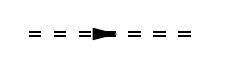
\begin{tikzpicture}[x=0.75pt,y=0.75pt,yscale=-1,xscale=1]
            %uncomment if require: \path (0,300); %set diagram left start at 0, and has height of 300
            
            %Straight Lines [id:da2580381812771073] 
            \draw  [dash pattern={on 4.5pt off 4.5pt}]  (167.71,167.57) -- (249.41,167.57) ;
            %Straight Lines [id:da1812296474143189] 
            \draw  [dash pattern={on 4.5pt off 4.5pt}]  (167.71,169.57) -- (249.41,169.57) ;
            %Straight Lines [id:da891236591561634] 
            \draw    (210.56,168.57) ;
            \draw [shift={(210.56,168.57)}, rotate = 180] [fill={rgb, 255:red, 0; green, 0; blue, 0 }  ][line width=0.08]  [draw opacity=0] (12,-3) -- (0,0) -- (12,3) -- cycle    ;
            \end{tikzpicture}
    \end{gathered} = \begin{gathered}
        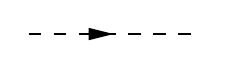
\begin{tikzpicture}[x=0.75pt,y=0.75pt,yscale=-1,xscale=1]
            %uncomment if require: \path (0,300); %set diagram left start at 0, and has height of 300
            
            %Straight Lines [id:da2580381812771073] 
            \draw  [dash pattern={on 4.5pt off 4.5pt}]  (167.71,167.57) -- (249.41,167.57) ;
            \draw [shift={(208.56,167.57)}, rotate = 180] [fill={rgb, 255:red, 0; green, 0; blue, 0 }  ][line width=0.08]  [draw opacity=0] (12,-3) -- (0,0) -- (12,3) -- cycle    ;
            \end{tikzpicture}
    \end{gathered} + \begin{gathered}
        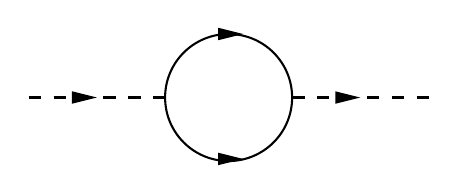
\begin{tikzpicture}[x=0.75pt,y=0.75pt,yscale=-1,xscale=1]
            %uncomment if require: \path (0,300); %set diagram left start at 0, and has height of 300
            
            %Straight Lines [id:da24576617158021508] 
            \draw  [dash pattern={on 4.5pt off 4.5pt}]  (100,125) -- (165.71,125) ;
            \draw [shift={(132.85,125)}, rotate = 180] [fill={rgb, 255:red, 0; green, 0; blue, 0 }  ][line width=0.08]  [draw opacity=0] (12,-3) -- (0,0) -- (12,3) -- cycle    ;
            %Shape: Circle [id:dp6762265906581268] 
            \draw   (165.71,125) .. controls (165.71,108.1) and (179.41,94.4) .. (196.31,94.4) .. controls (213.21,94.4) and (226.91,108.1) .. (226.91,125) .. controls (226.91,141.9) and (213.21,155.6) .. (196.31,155.6) .. controls (179.41,155.6) and (165.71,141.9) .. (165.71,125) -- cycle ;
            %Straight Lines [id:da46135211886694005] 
            \draw  [dash pattern={on 4.5pt off 4.5pt}]  (226.91,125) -- (292.62,125) ;
            \draw [shift={(259.76,125)}, rotate = 180] [fill={rgb, 255:red, 0; green, 0; blue, 0 }  ][line width=0.08]  [draw opacity=0] (12,-3) -- (0,0) -- (12,3) -- cycle    ;
            %Straight Lines [id:da09338269031575619] 
            \draw    (203.31,94.4) ;
            \draw [shift={(203.31,94.4)}, rotate = 180] [fill={rgb, 255:red, 0; green, 0; blue, 0 }  ][line width=0.08]  [draw opacity=0] (12,-3) -- (0,0) -- (12,3) -- cycle    ;
            %Straight Lines [id:da4104133236840597] 
            \draw    (203.31,154.6) ;
            \draw [shift={(203.31,154.6)}, rotate = 180] [fill={rgb, 255:red, 0; green, 0; blue, 0 }  ][line width=0.08]  [draw opacity=0] (12,-3) -- (0,0) -- (12,3) -- cycle    ;
            \end{tikzpicture}                  
    \end{gathered},
    \label{eq:bcs-cooper-2nd-propagator}
\end{equation}
正好就是\eqref{eq:bcs-action-delta2}对应的传播子(负号可以解释成闭合费米子回线导致的)。
注意到$\sum_{k} G_{k+q} G_{-k}$也出现在了\eqref{eq:bcs-cooper-pair-correlation}中,这当然不是偶然的:通过图形很容易发现电子的梯形图近似实际上就是库伯对的环形图近似(或者,注意到电子的梯形图近似\eqref{eq:bcs-four-e-vertex-eff}修正了$g$,而$\int \dd{\tau} \sum_q 1/g \bar{\Delta}_q \Delta_q$正好是未经过相互作用修饰的库伯对的作用量),而\eqref{eq:bcs-cooper-2nd-propagator}是库伯对的环形图近似的最多保留两个顶角的低阶项。
以上两种等价的近似实际上也等价于只计算库伯对的最低阶自能,即认为电子-库伯对转化顶角导致的自能修正为
\begin{equation}
    - \Sigma_q = \frac{1}{V \beta} \sum_{k} (- G^\text{e}_{k+q}) (- G^\text{e}_{-k}).
\end{equation}
按照\eqref{eq:bcs-cooper-pair-correlation-strange-part},这就是
\begin{equation}
    \Sigma_q = \frac{1}{V} \sum_{\vb*{p}} \frac{1 - f(\xi_{\vb*{p}}) - f(\xi_{\vb*{p}+\vb*{q}})}{\ii q^0 - \xi_{\vb*{p}} - \xi_{\vb*{p} + \vb*{q}}}.
\end{equation}

我们现在切换回实空间。前面说过,能量最低的场构型中$\Delta$在时间和空间上都是均匀的,即参与库伯配对的两个电子动量基本上只差一个负号,从而,基态附近的$\vb*{q}$通常都很小,类似的$q^0$也很小,这样我们将对$\vb*{q}$展开,由于考虑的是s波超导,
\[
    \Sigma_{q} = \Sigma_{0} + \ii q^0 \eval{\pdv{\Sigma_{q}}{(\ii q^0)}}_{q=0} + \frac{1}{6} \abs*{\vb*{q}}^2 \laplacian_{\vb*{q}} \Sigma_{q} |_{q=0} + \cdots,
\]
但是更进一步的计算会发现
\[
    \eval{\pdv{\Sigma_{q}}{(\ii q^0)}}_{q=0} = 
\]
因此最后通过适当地重新定义$\Delta$以囊括一些因子,就能够得到
\begin{equation}
    S_{\Delta^2} = \int \dd{\tau} \int \dd[3]{\vb*{r}} \left( \frac{c}{2} \abs{\grad{\Delta}}^2 + \frac{r}{2} \abs{\Delta}^2 \right).
\end{equation}
\eqref{eq:bcs-kernal-expansion}中的$n=2$项则是$\Delta$的一个四阶项,同样,它也有$\abs{\vb*{q}}^2$和$\ii q^0$的依赖,但是既然我们认为$\vb*{q}$和$\Delta$都是小量,实际上只有$\abs{\Delta}^4$的量级是足够客观的,于是可以直接写出
\begin{equation}
    S = \int \dd{\tau} \int \dd[3]{\vb*{r}} \left( \frac{c}{2} \abs{\grad{\Delta}}^2 + \frac{r}{2} \abs{\Delta}^2 + \frac{u}{4} \abs{\Delta}^4 \right).
    \label{eq:bcs-copper-theory}
\end{equation}
% TODO: u要是正的

我们可以发现以上计算过程给出的有效作用量可以有量子涨落,但是自身没有动力学,或者说BCS序参量$\Delta$在没有外场时没有时间演化。

在温度稍微高一些时量子涨落可以忽略,此时我们得到所谓的\concept{s波超导体的经典金斯堡-朗道理论}
\begin{equation}
    S = \beta \int \dd[3]{\vb*{r}} \left( \frac{c}{2} \abs{\grad{\Delta}}^2 + \frac{r}{2} \abs{\Delta}^2 + \frac{u}{4} \abs{\Delta}^4 \right).
\end{equation}
这是朗道

\subsection{s波BCS超导体的电磁学性能}

\subsubsection{伦敦方程}

\begin{back}{规范场}{gauge-field}
    设$G$是一个李群,$S$是它的一个表示,使用参数$\alpha$标记。
    在底流形$M$上每一点放置一个$S$,并让$\alpha$可以随着时空点的不同而变化。
    设$M$上的场$\psi(x)$的目标空间(即某一点上场值的取值范围)携带了$S$的一个表示。
    如此构造之后,就能够定义规范变换
    \[
        \psi'(x) = S(x) \psi(x).
    \]

    现在设我们有了一个关于$\psi(x)$的拉氏量$\mathcal{L}_{\psi}$。如果我们希望让$\mathcal{L}_{\psi}$成为\emph{规范不变}的,即如果另外找任意一个$S'(x)$,根据$S'(x)$做规范变换,拉氏量不变,那么可以验证,只需要将$\mathcal{L}_{\psi}$中的所有导数替换为以$-\ii e A_\mu$为联络的协变导数即可,其中$A_\mu(x)$是$x$点的$S(x)$的$\alpha(x)$发生无穷小变化而产生的$S(x)$的变化,从而是$S$表示的生成元的一个线性组合。

    因此我们获得了一种批量生产拉氏量的方式:给定一些场,选取特定的规范群$G$,使得前述的场能够携带$G$的某个表示,即可自动生成一个规范场(实际上是一个多分量的场),将前述的各种场耦合在一起。
    高能物理中最为成功的标准模型就是通过这种方式构造出来的。
    在凝聚态物理中,以上构造方式也可以大大简化推导,例如要推导BCS理论中库伯对的作用量,我们只需要知道库伯对也携带了规范群$U(1)$的某个表示,就知道了它和电磁场耦合的方式,从而无需从与电磁场耦合的库伦排斥电子气的场论出发从头推导一遍就能够知道库伯对和电磁场耦合的方式。
    唯一尚有待分析的是一个库伯对的电荷量,但是这也可以通过电荷守恒很自然地得到(库伯对的流和对应的电子的流必须给出一样的电荷流)。

    引入规范场的一个直接结果是与规范场耦合的粒子(即场$\psi$产生的粒子)获得Berry相位。

    虽然以上构造是在一个底流形$M$上进行的,但是把$M$换成一个格点系统也可以;不过此时要注意,规范联络应该定义在$\psi$场对应的粒子能够跃迁的\emph{边}上而不是格点上,虽然诸$S(x)$还是定义在格点上的。
\end{back}

\subsection{超导和超流}

\eqref{eq:bcs-copper-theory}是一个有排斥相互作用的玻色场论。
这样的系统可能会呈现一个\concept{超流}相。这是BCS超导的一个直观解释:电子配对形成的库伯对组成的玻色流体在低温下进入超流相,从而可以没有阻碍地移动。

\begin{back}{近独立玻色气体的玻色-爱因斯坦凝聚}{bose-gas-bec}
    近独立玻色气体的基态是所谓的\concept{玻色-爱因斯坦凝聚}。可以从玻色分布函数的形式看出这一点:$\epsilon < \mu$时分布函数就是负的,不物理,从而一定有$\epsilon \geq \mu$。
    而另一方面,简单的积分就能够说明,$\epsilon > \mu$这部分能级能够容纳的玻色子数目是有限的,随着温度降低而降低。
    因此,在零温下,压倒性多数的玻色子停留在$\epsilon = \mu$能级上,进一步的分析表明它们构成一个相干态。
\end{back}

\subsubsection{玻色液体的超流相}

在超流相中,粒子数流密度为
\[
    \vb*{j} = \frac{\ii}{2m} ( \psi \grad{\bar{\psi}} - \bar{\psi} \grad{\psi} ),
\]
在$U(1)$对称性破缺相中就有
\begin{equation}
    \vb*{j} = \frac{\rho_0}{m} \grad{\theta}.
\end{equation}
这就意味着,$U(1)$对称性破缺相中,只需要序参量$\theta$——也就是玻色子场的相角——在空间上有一个涨落,就\emph{一定}会有粒子数流密度,而且是没完没了、不会衰减的流密度。
因此$U(1)$对称性破缺相就是\concept{超流相}。

\subsubsection{超流中的拓扑激发}

\subsection{BCS以外的超导机制}

配对机制可以不是声子介导的有效吸引相互作用。

有效吸引相互作用在一些时候可能不能被看成瞬时的。如果一个声子被创生之后可以在空间中激发出别的声子,且声子能够在材料中产生诸如电流等涉及范围较大且短时间内不容易被弛豫掉的模式,那么有效的电子-电子相互作用就根本不应该看成瞬时的。

\section{相邻自旋-自旋相互作用导致的二维正方晶格的反铁磁长程序}\label{sec:spin-spin-nn-interaction-sdw}

\subsection{二维正方晶格上的自旋}

\begin{figure}
    \centering
    \subfigure[自旋密度波]{
        

\tikzset{every picture/.style={line width=0.75pt}} %set default line width to 0.75pt        

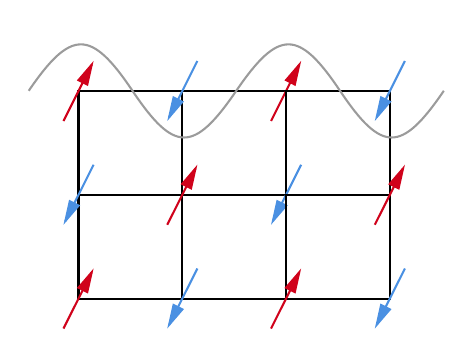
\begin{tikzpicture}[x=0.75pt,y=0.75pt,yscale=-1,xscale=1]
%uncomment if require: \path (0,300); %set diagram left start at 0, and has height of 300

%Shape: Square [id:dp7968380272014384] 
\draw   (148,62) -- (198,62) -- (198,112) -- (148,112) -- cycle ;
%Shape: Square [id:dp08936498453558128] 
\draw   (98,62) -- (148,62) -- (148,112) -- (98,112) -- cycle ;
%Shape: Square [id:dp6338164799723338] 
\draw   (98,112) -- (148,112) -- (148,162) -- (98,162) -- cycle ;
%Shape: Square [id:dp5647790600566112] 
\draw   (148,112) -- (198,112) -- (198,162) -- (148,162) -- cycle ;
%Straight Lines [id:da4505706138663077] 
\draw [color={rgb, 255:red, 208; green, 2; blue, 27 }  ,draw opacity=1 ]   (90.75,76.46) -- (104.35,49.33) ;
\draw [shift={(105.25,47.54)}, rotate = 476.63] [fill={rgb, 255:red, 208; green, 2; blue, 27 }  ,fill opacity=1 ][line width=0.08]  [draw opacity=0] (12,-3) -- (0,0) -- (12,3) -- cycle    ;
%Straight Lines [id:da8302639980131186] 
\draw [color={rgb, 255:red, 74; green, 144; blue, 226 }  ,draw opacity=1 ]   (155.25,47.54) -- (141.65,74.67) ;
\draw [shift={(140.75,76.46)}, rotate = 296.63] [fill={rgb, 255:red, 74; green, 144; blue, 226 }  ,fill opacity=1 ][line width=0.08]  [draw opacity=0] (12,-3) -- (0,0) -- (12,3) -- cycle    ;
%Straight Lines [id:da07392319534895608] 
\draw [color={rgb, 255:red, 208; green, 2; blue, 27 }  ,draw opacity=1 ]   (140.75,126.46) -- (154.35,99.33) ;
\draw [shift={(155.25,97.54)}, rotate = 476.63] [fill={rgb, 255:red, 208; green, 2; blue, 27 }  ,fill opacity=1 ][line width=0.08]  [draw opacity=0] (12,-3) -- (0,0) -- (12,3) -- cycle    ;
%Straight Lines [id:da29949826504712806] 
\draw [color={rgb, 255:red, 208; green, 2; blue, 27 }  ,draw opacity=1 ]   (90.75,176.46) -- (104.35,149.33) ;
\draw [shift={(105.25,147.54)}, rotate = 476.63] [fill={rgb, 255:red, 208; green, 2; blue, 27 }  ,fill opacity=1 ][line width=0.08]  [draw opacity=0] (12,-3) -- (0,0) -- (12,3) -- cycle    ;
%Straight Lines [id:da10136846066630589] 
\draw [color={rgb, 255:red, 208; green, 2; blue, 27 }  ,draw opacity=1 ]   (190.75,76.46) -- (204.35,49.33) ;
\draw [shift={(205.25,47.54)}, rotate = 476.63] [fill={rgb, 255:red, 208; green, 2; blue, 27 }  ,fill opacity=1 ][line width=0.08]  [draw opacity=0] (12,-3) -- (0,0) -- (12,3) -- cycle    ;
%Straight Lines [id:da18679469569417329] 
\draw [color={rgb, 255:red, 74; green, 144; blue, 226 }  ,draw opacity=1 ]   (105.25,97.54) -- (91.65,124.67) ;
\draw [shift={(90.75,126.46)}, rotate = 296.63] [fill={rgb, 255:red, 74; green, 144; blue, 226 }  ,fill opacity=1 ][line width=0.08]  [draw opacity=0] (12,-3) -- (0,0) -- (12,3) -- cycle    ;
%Straight Lines [id:da9509291375625459] 
\draw [color={rgb, 255:red, 74; green, 144; blue, 226 }  ,draw opacity=1 ]   (155.25,147.54) -- (141.65,174.67) ;
\draw [shift={(140.75,176.46)}, rotate = 296.63] [fill={rgb, 255:red, 74; green, 144; blue, 226 }  ,fill opacity=1 ][line width=0.08]  [draw opacity=0] (12,-3) -- (0,0) -- (12,3) -- cycle    ;
%Shape: Square [id:dp7989800051587621] 
\draw   (198,62) -- (248,62) -- (248,112) -- (198,112) -- cycle ;
%Straight Lines [id:da025654938728039145] 
\draw [color={rgb, 255:red, 74; green, 144; blue, 226 }  ,draw opacity=1 ]   (205.25,97.54) -- (191.65,124.67) ;
\draw [shift={(190.75,126.46)}, rotate = 296.63] [fill={rgb, 255:red, 74; green, 144; blue, 226 }  ,fill opacity=1 ][line width=0.08]  [draw opacity=0] (12,-3) -- (0,0) -- (12,3) -- cycle    ;
%Shape: Square [id:dp21923612897643863] 
\draw   (198,112) -- (248,112) -- (248,162) -- (198,162) -- cycle ;
%Straight Lines [id:da2934635233522882] 
\draw [color={rgb, 255:red, 208; green, 2; blue, 27 }  ,draw opacity=1 ]   (190.75,176.46) -- (204.35,149.33) ;
\draw [shift={(205.25,147.54)}, rotate = 476.63] [fill={rgb, 255:red, 208; green, 2; blue, 27 }  ,fill opacity=1 ][line width=0.08]  [draw opacity=0] (12,-3) -- (0,0) -- (12,3) -- cycle    ;
%Straight Lines [id:da9412499087817388] 
\draw [color={rgb, 255:red, 74; green, 144; blue, 226 }  ,draw opacity=1 ]   (255.25,47.54) -- (241.65,74.67) ;
\draw [shift={(240.75,76.46)}, rotate = 296.63] [fill={rgb, 255:red, 74; green, 144; blue, 226 }  ,fill opacity=1 ][line width=0.08]  [draw opacity=0] (12,-3) -- (0,0) -- (12,3) -- cycle    ;
%Straight Lines [id:da18617934942542336] 
\draw [color={rgb, 255:red, 74; green, 144; blue, 226 }  ,draw opacity=1 ]   (255.25,147.54) -- (241.65,174.67) ;
\draw [shift={(240.75,176.46)}, rotate = 296.63] [fill={rgb, 255:red, 74; green, 144; blue, 226 }  ,fill opacity=1 ][line width=0.08]  [draw opacity=0] (12,-3) -- (0,0) -- (12,3) -- cycle    ;
%Straight Lines [id:da24257455825409324] 
\draw [color={rgb, 255:red, 208; green, 2; blue, 27 }  ,draw opacity=1 ]   (240.75,126.46) -- (254.35,99.33) ;
\draw [shift={(255.25,97.54)}, rotate = 476.63] [fill={rgb, 255:red, 208; green, 2; blue, 27 }  ,fill opacity=1 ][line width=0.08]  [draw opacity=0] (12,-3) -- (0,0) -- (12,3) -- cycle    ;
%Shape: Sine Wave Form [id:dp4769190459095818] 
\draw  [color={rgb, 255:red, 155; green, 155; blue, 155 }  ,draw opacity=1 ] (74,61.91) .. controls (94.35,32.16) and (103.94,32) .. (123.99,61.91) .. controls (144.06,91.82) and (153.47,92) .. (174,61.91) ;
%Shape: Sine Wave Form [id:dp8043046043167636] 
\draw  [color={rgb, 255:red, 155; green, 155; blue, 155 }  ,draw opacity=1 ] (174,61.91) .. controls (194.35,32.16) and (203.94,32) .. (223.99,61.91) .. controls (244.06,91.82) and (253.47,92) .. (274,61.91) ;




\end{tikzpicture}      
    }
    \subfigure[SDW形成后的两条子格子]{
        

\tikzset{every picture/.style={line width=0.75pt}} %set default line width to 0.75pt        

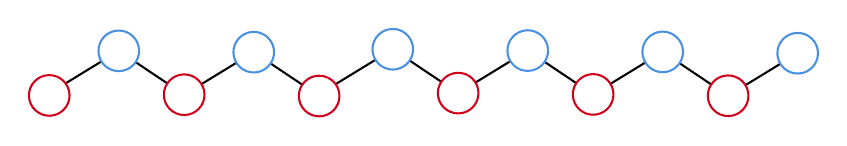
\begin{tikzpicture}[x=0.75pt,y=0.75pt,yscale=-1,xscale=1]
%uncomment if require: \path (0,300); %set diagram left start at 0, and has height of 300

%Straight Lines [id:da5978907907830429] 
\draw    (101.11,108.45) -- (132.62,129.57) ;
%Straight Lines [id:da6479636898097754] 
\draw    (166.14,109.09) -- (197.65,130.21) ;
%Straight Lines [id:da20799022198939388] 
\draw    (233.12,107.68) -- (264.64,128.81) ;
%Straight Lines [id:da7588059918995707] 
\draw    (298.15,108.32) -- (329.66,129.45) ;
%Straight Lines [id:da04554146426034689] 
\draw    (363.18,108.96) -- (394.69,130.09) ;
%Straight Lines [id:da6866628962323054] 
\draw    (67.6,128.94) -- (101.11,108.45) ;
%Shape: Circle [id:dp960424577904551] 
\draw  [color={rgb, 255:red, 208; green, 2; blue, 27 }  ,draw opacity=1 ][fill={rgb, 255:red, 255; green, 255; blue, 255 }  ,fill opacity=1 ] (57.83,130.14) .. controls (57.72,124.74) and (62.01,120.27) .. (67.41,120.15) .. controls (72.82,120.04) and (77.29,124.33) .. (77.4,129.73) .. controls (77.51,135.13) and (73.23,139.61) .. (67.82,139.72) .. controls (62.42,139.83) and (57.95,135.54) .. (57.83,130.14) -- cycle ;
%Shape: Circle [id:dp278517736754311] 
\draw  [color={rgb, 255:red, 74; green, 144; blue, 226 }  ,draw opacity=1 ][fill={rgb, 255:red, 255; green, 255; blue, 255 }  ,fill opacity=1 ] (91.32,108.65) .. controls (91.21,103.25) and (95.5,98.78) .. (100.9,98.67) .. controls (106.31,98.55) and (110.78,102.84) .. (110.89,108.24) .. controls (111.01,113.65) and (106.72,118.12) .. (101.31,118.23) .. controls (95.91,118.35) and (91.44,114.06) .. (91.32,108.65) -- cycle ;
%Straight Lines [id:da8951114155214333] 
\draw    (132.62,129.57) -- (166.14,109.09) ;
%Shape: Circle [id:dp6119193772576137] 
\draw  [color={rgb, 255:red, 208; green, 2; blue, 27 }  ,draw opacity=1 ][fill={rgb, 255:red, 255; green, 255; blue, 255 }  ,fill opacity=1 ] (122.84,129.78) .. controls (122.73,124.38) and (127.02,119.9) .. (132.42,119.79) .. controls (137.82,119.68) and (142.29,123.97) .. (142.41,129.37) .. controls (142.52,134.77) and (138.23,139.25) .. (132.83,139.36) .. controls (127.43,139.47) and (122.95,135.18) .. (122.84,129.78) -- cycle ;
%Shape: Circle [id:dp7508217961101133] 
\draw  [color={rgb, 255:red, 74; green, 144; blue, 226 }  ,draw opacity=1 ][fill={rgb, 255:red, 255; green, 255; blue, 255 }  ,fill opacity=1 ] (156.35,109.29) .. controls (156.24,103.89) and (160.53,99.42) .. (165.93,99.3) .. controls (171.33,99.19) and (175.81,103.48) .. (175.92,108.88) .. controls (176.03,114.29) and (171.74,118.76) .. (166.34,118.87) .. controls (160.94,118.98) and (156.47,114.7) .. (156.35,109.29) -- cycle ;
%Straight Lines [id:da6824105788244417] 
\draw    (199.61,128.17) -- (233.12,107.68) ;
%Shape: Circle [id:dp6550057353578134] 
\draw  [color={rgb, 255:red, 208; green, 2; blue, 27 }  ,draw opacity=1 ][fill={rgb, 255:red, 255; green, 255; blue, 255 }  ,fill opacity=1 ] (187.87,130.42) .. controls (187.75,125.01) and (192.04,120.54) .. (197.45,120.43) .. controls (202.85,120.32) and (207.32,124.6) .. (207.43,130.01) .. controls (207.55,135.41) and (203.26,139.88) .. (197.86,140) .. controls (192.45,140.11) and (187.98,135.82) .. (187.87,130.42) -- cycle ;
%Shape: Circle [id:dp2789113887024053] 
\draw  [color={rgb, 255:red, 74; green, 144; blue, 226 }  ,draw opacity=1 ][fill={rgb, 255:red, 255; green, 255; blue, 255 }  ,fill opacity=1 ] (223.34,107.89) .. controls (223.22,102.49) and (227.51,98.01) .. (232.92,97.9) .. controls (238.32,97.79) and (242.79,102.08) .. (242.9,107.48) .. controls (243.02,112.88) and (238.73,117.35) .. (233.33,117.47) .. controls (227.92,117.58) and (223.45,113.29) .. (223.34,107.89) -- cycle ;
%Straight Lines [id:da9835803759861903] 
\draw [color={rgb, 255:red, 0; green, 0; blue, 0 }  ,draw opacity=1 ][fill={rgb, 255:red, 208; green, 2; blue, 27 }  ,fill opacity=1 ]   (264.64,128.81) -- (298.15,108.32) ;
%Shape: Circle [id:dp3465061446468005] 
\draw  [color={rgb, 255:red, 208; green, 2; blue, 27 }  ,draw opacity=1 ][fill={rgb, 255:red, 255; green, 255; blue, 255 }  ,fill opacity=1 ] (254.85,129.02) .. controls (254.74,123.61) and (259.03,119.14) .. (264.43,119.03) .. controls (269.83,118.91) and (274.31,123.2) .. (274.42,128.61) .. controls (274.53,134.01) and (270.24,138.48) .. (264.84,138.59) .. controls (259.44,138.71) and (254.97,134.42) .. (254.85,129.02) -- cycle ;
%Shape: Circle [id:dp2919589177523425] 
\draw  [color={rgb, 255:red, 74; green, 144; blue, 226 }  ,draw opacity=1 ][fill={rgb, 255:red, 255; green, 255; blue, 255 }  ,fill opacity=1 ] (288.36,108.53) .. controls (288.25,103.12) and (292.54,98.65) .. (297.94,98.54) .. controls (303.35,98.43) and (307.82,102.71) .. (307.93,108.12) .. controls (308.05,113.52) and (303.76,117.99) .. (298.35,118.11) .. controls (292.95,118.22) and (288.48,113.93) .. (288.36,108.53) -- cycle ;
%Straight Lines [id:da3388603264007448] 
\draw    (329.66,129.45) -- (363.18,108.96) ;
%Shape: Circle [id:dp22822608286568746] 
\draw  [color={rgb, 255:red, 208; green, 2; blue, 27 }  ,draw opacity=1 ][fill={rgb, 255:red, 255; green, 255; blue, 255 }  ,fill opacity=1 ] (319.88,129.65) .. controls (319.77,124.25) and (324.06,119.78) .. (329.46,119.66) .. controls (334.86,119.55) and (339.33,123.84) .. (339.45,129.24) .. controls (339.56,134.65) and (335.27,139.12) .. (329.87,139.23) .. controls (324.47,139.35) and (319.99,135.06) .. (319.88,129.65) -- cycle ;
%Shape: Circle [id:dp9731435281234146] 
\draw  [color={rgb, 255:red, 74; green, 144; blue, 226 }  ,draw opacity=1 ][fill={rgb, 255:red, 255; green, 255; blue, 255 }  ,fill opacity=1 ] (353.39,109.17) .. controls (353.28,103.76) and (357.57,99.29) .. (362.97,99.18) .. controls (368.37,99.06) and (372.85,103.35) .. (372.96,108.76) .. controls (373.07,114.16) and (368.78,118.63) .. (363.38,118.74) .. controls (357.98,118.86) and (353.51,114.57) .. (353.39,109.17) -- cycle ;
%Straight Lines [id:da7953208412330044] 
\draw    (394.69,130.09) -- (428.2,109.6) ;
%Shape: Circle [id:dp6293699664956078] 
\draw  [color={rgb, 255:red, 208; green, 2; blue, 27 }  ,draw opacity=1 ][fill={rgb, 255:red, 255; green, 255; blue, 255 }  ,fill opacity=1 ] (384.91,130.29) .. controls (384.79,124.89) and (389.08,120.42) .. (394.49,120.3) .. controls (399.89,120.19) and (404.36,124.48) .. (404.48,129.88) .. controls (404.59,135.29) and (400.3,139.76) .. (394.9,139.87) .. controls (389.49,139.98) and (385.02,135.7) .. (384.91,130.29) -- cycle ;
%Shape: Circle [id:dp5339722494647174] 
\draw  [color={rgb, 255:red, 74; green, 144; blue, 226 }  ,draw opacity=1 ][fill={rgb, 255:red, 255; green, 255; blue, 255 }  ,fill opacity=1 ] (418.42,109.8) .. controls (418.31,104.4) and (422.6,99.93) .. (428,99.82) .. controls (433.4,99.7) and (437.87,103.99) .. (437.99,109.39) .. controls (438.1,114.8) and (433.81,119.27) .. (428.41,119.38) .. controls (423.01,119.5) and (418.53,115.21) .. (418.42,109.8) -- cycle ;




\end{tikzpicture}

    }
    \caption{二维正方晶格上的反铁磁序}
\end{figure}

现在考虑一个二维正方晶格,它可以有一个反铁磁相,也即,相邻格点的自旋倾向于变得反平行,或者说形成一个自旋密度波。
一种能够产生反铁磁序的哈密顿量为
\begin{equation}
    {H} = \sum_{\vb*{k}, \alpha} \xi_{\vb*{k}} {c}_{\vb*{k} \alpha}^\dagger {c}_{\vb*{k} \alpha} + J \sum_{\pair{\vb*{i}, \vb*{j}}} {\vb*{S}}_{\vb*{i}} \cdot {\vb*{S}}_{\vb*{j}},
    \label{eq:2dim-square-spin}
\end{equation}
其中
\begin{equation}
    {\vb*{S}}_{\vb*{i}} = \sum_{\alpha, \beta} {c}^\dagger_{\vb*{i} \alpha} \vb*{\sigma}_{\alpha \beta} {c}_{\vb*{i} \beta}
    \label{eq:spin-wave-order-parameter}
\end{equation}
为格点$i$的自旋矢量。这个模型本身其实并不非常现实,因为自旋相互作用通常来自交换能,但是交换能通常在绝缘系统中比较重要,那么就不应该有一个动能项。
设反铁磁序的序参量为$\vb*{\phi}$,一个不错的选择是
\begin{equation}
    \expval*{{\vb*{S}}_{\vb*{i}}} = (-1)^{\vb*{i}} \vb*{\phi},
\end{equation}
这里的$(-1)^{\vb*{i}}$实际上是一种滥用记号:它实际上是
\[
    (-1)^{\vb*{i}} = (-1)^{i_x + i_y}
\]
的简写。为了方便起见,我们把$(i_x + i_y)$为奇数的格点的全体记为$A$,将$(i_x + i_y)$为偶数的格点的全体记为$B$,于是$A$中任何一个格点的近邻格点都在$B$中,反之亦然。
如果$\vb*{\phi}$非零,那么显然$\expval*{{\vb*{S}}_{\vb*{i}}}$在$i \in A$时和$\expval*{{\vb*{S}}_{\vb*{i}}}$在$i \in B$时差一个负号,即相邻的自旋一定是反向的,正好意味着形成了反铁磁序。

不失一般性地令晶格常数为1,则第一布里渊区为$[-\pi, \pi)^2$。在形成了一个完整的反铁磁序之后序参量$\Delta$的周期应该是两个格点,于是应有$\vb*{Q}=(\pi, \pi)$。

\subsection{平均场近似}

在\eqref{eq:2dim-square-spin}中做平均场近似
\begin{equation}
    \vb*{{S}}_{\vb*{i}} \cdot \vb*{{S}}_{\vb*{j}} = \expval*{\vb*{{S}}_{\vb*{i}}} \cdot \vb*{{S}}_{\vb*{j}} + \vb*{{S}}_{\vb*{i}} \cdot \expval*{\vb*{{S}}_{\vb*{j}}} - \expval*{\vb*{{S}}_{\vb*{i}}} \cdot \expval*{\vb*{{S}}_{\vb*{j}}},
\end{equation}
忽略平均场近似引入的常数项(我们这里不做自洽计算而只是分析相变点具有的性质),自旋相互作用项为
\[
    \begin{aligned}
        {H}_\text{int} = J \sum_{\pair{\vb*{i}, \vb*{j}}} {\vb*{S}}_{\vb*{i}} \cdot {\vb*{S}}_{\vb*{j}} &\sim J \sum_{\pair{\vb*{i}, \vb*{j}}} (\expval*{\vb*{{S}}_{\vb*{i}}} \cdot \vb*{{S}}_{\vb*{j}} + \vb*{{S}}_{\vb*{i}} \cdot \expval*{\vb*{{S}}_{\vb*{j}}}) \\
        &= 2 J \sum_{\pair{\vb*{i}, \vb*{j}}} \expval*{\vb*{{S}}_{\vb*{j}}} \cdot \vb*{{S}}_{\vb*{i}} \\
        &= J \sum_{\vb*{i}} \sum_{\vb*{j} \in \text{nn of } \vb*{i}} \expval*{\vb*{{S}}_{\vb*{j}}} \cdot \vb*{{S}}_{\vb*{i}},
    \end{aligned}
\]
其中nn表示“最近邻”,第二个等号中因子2消失了是因为$\pair{\vb*{i}, \vb*{j}}$对一对近邻只求和一次,而第三行中一对近邻实际上被求和了两次。
代入\eqref{eq:spin-wave-order-parameter},注意到两个相邻格点的$(-1)^{\vb*{i}}$差一个负号,有
\[
    \begin{aligned}
        {H}_\text{int} &= J \sum_{\vb*{i}} \sum_{\vb*{j} \in \text{nn of } \vb*{i}} (-1)^{\vb*{j}} \vb*{\phi} \cdot \vb*{{S}}_{\vb*{i}} \\
        &= - J \sum_{\vb*{i}} (-1)^{\vb*{i}} \sum_{\vb*{j} \in \text{nn of } \vb*{i}} \vb*{\phi} \cdot \vb*{{S}}_{\vb*{i}},
    \end{aligned}
\]
由于系统具有自旋旋转不变性,不失一般性地要求$\vb*{\phi}$指向$z$轴,并设
\begin{equation}
    \Delta = 4 J \phi,
\end{equation}
则
\begin{equation}
    {H}_\text{int} = - \sum_{\vb*{i}} (-1)^{\vb*{i}} {S}_{\vb*{i}}^z \Delta = - \sum_{\vb*{i}} (-1)^{\vb*{i}} \Delta ({c}_{\vb*{i} \uparrow}^\dagger {c}_{\vb*{i} \uparrow} - {c}_{\vb*{i} \downarrow}^\dagger {c}_{\vb*{i} \downarrow}).
\end{equation}
设$\vb*{Q}=(\pi, \pi)$,则相互作用哈密顿量可以写成以下傅里叶变换的形式: 
\begin{equation}
    {H}_\text{int} = - \sum_{\vb*{i}} \ee^{\ii \vb*{Q} \cdot \vb*{R}_i} \Delta ({c}_{\vb*{i} \uparrow}^\dagger {c}_{\vb*{i} \uparrow} - {c}_{\vb*{i} \downarrow}^\dagger {c}_{\vb*{i} \downarrow}) 
    = - \Delta \sum_{\vb*{k}} ({c}_{(\vb*{k} + \vb*{Q})\uparrow}^\dagger {c}_{\vb*{k} \uparrow} - {c}_{(\vb*{k}+\vb*{Q}) \downarrow}^\dagger {c}_{\vb*{k} \downarrow}).
\end{equation}
于是最后平均场哈密顿量就是
\begin{equation}
    {H}_\text{MF} = \sum_{\vb*{k}, \alpha} (\xi_{\vb*{k}} {c}_{\vb*{k} \alpha}^\dagger {c}_{\vb*{k} \alpha} - \alpha \Delta {c}_{(\vb*{k} + \vb*{Q}) \alpha}^\dagger {c}_{\vb*{k} \alpha}).
    \label{eq:2dim-square-spin-mf}
\end{equation}
这里指定$\uparrow$对应$1$,$\downarrow$对应$-1$,虽然电子的自旋为$\pm 1/2$而不是$\pm 1$。
\eqref{eq:2dim-square-spin-mf}两边乘上2,并注意对$\vb*{k}$求和等价于对$\vb*{k}+Q$求和,且$\vb*{k}$等价于$\vb*{k}+2\vb*{Q}$,\eqref{eq:2dim-square-spin-mf}给出的能谱等价于以下矩阵
\[
    \pmqty{\xi_{\vb*{k}} & - \alpha \Delta \\ - \alpha \Delta & \xi_{\vb*{k} + \vb*{Q}}}
\]
的本征值,也就是
\begin{equation}
    E_{\vb*{k}} = \frac{\xi_{\vb*{k}} + \xi_{\vb*{k} + \vb*{Q}}}{2} \pm \sqrt{\frac{(\xi_{\vb*{k}} - \xi_{\vb*{k}+\vb*{Q}})^2}{4} + \alpha^2 \Delta^2}.
\end{equation}
这样可以得到两条能带,在$\Delta$为零时它们可以交叉,在$\Delta$不为零时能带交叉的部位就打开了一个能隙。

\subsection{热点和它附近的低能有效理论}

\eqref{eq:2dim-square-spin-mf}是\eqref{eq:2dim-square-spin}在反铁磁序相的一个有效理论。反铁磁序破缺了晶格上的平移不变性,因为反铁磁序状态中每个晶格和临近的晶格的自旋差一个负号。
反铁磁序还保留了一部分平移不变性:子格点$A$和$B$上仍有平移不变性,这两个子格点对应的倒格矢都是$\vb*{Q}$。
这样,\eqref{eq:2dim-square-spin-mf}的第一布里渊区是
\[
    \abs{k_x} + \abs{k_y} \leq \pi,
\]
这是\eqref{eq:2dim-square-spin}的第一布里渊区折叠之后得到的。
布里渊区变小当然是因为原胞变大了——从单个格点变成了一个$A$格点加上一个$B$格点。(见\autoref{sec:quasi-particle-spectrum})

\begin{figure}
    \centering
    \subfigure[一个单带模型的第一布里渊区和费米面]{
        

\tikzset{every picture/.style={line width=0.75pt}} %set default line width to 0.75pt        

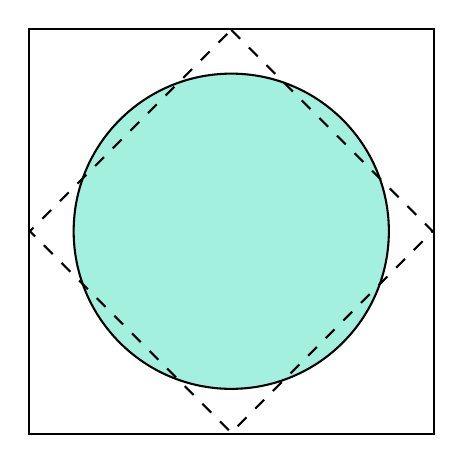
\begin{tikzpicture}[x=0.75pt,y=0.75pt,yscale=-1,xscale=1]
%uncomment if require: \path (0,300); %set diagram left start at 0, and has height of 300

%Shape: Square [id:dp2502427835904639] 
\draw   (241.83,21.67) -- (437,21.67) -- (437,216.83) -- (241.83,216.83) -- cycle ;
%Shape: Circle [id:dp1839510682473804] 
\draw  [fill={rgb, 255:red, 80; green, 227; blue, 194 }  ,fill opacity=0.52 ] (263.48,119.25) .. controls (263.48,77.31) and (297.48,43.31) .. (339.42,43.31) .. controls (381.36,43.31) and (415.35,77.31) .. (415.35,119.25) .. controls (415.35,161.19) and (381.36,195.19) .. (339.42,195.19) .. controls (297.48,195.19) and (263.48,161.19) .. (263.48,119.25) -- cycle ;
%Shape: Square [id:dp70425401409973] 
\draw  [dash pattern={on 4.5pt off 4.5pt}] (339.42,22.25) -- (436.42,119.25) -- (339.42,216.25) -- (242.42,119.25) -- cycle ;




\end{tikzpicture}

    }
    \subfigure[将格点划分为A格点和B格点之后的第一布里渊区和费米面,注意费米面和折叠了的第一布里渊区相交]{
        

\tikzset{every picture/.style={line width=0.75pt}} %set default line width to 0.75pt        

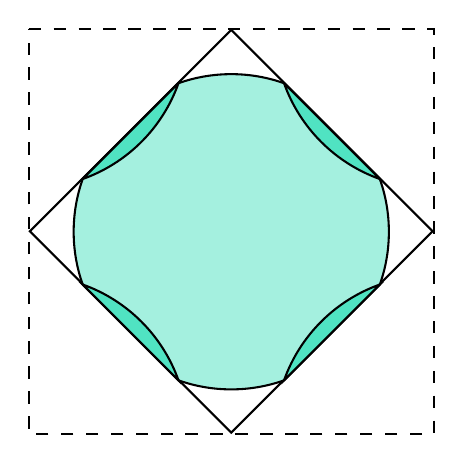
\begin{tikzpicture}[x=0.75pt,y=0.75pt,yscale=-1,xscale=1]
%uncomment if require: \path (0,259); %set diagram left start at 0, and has height of 259

%Shape: Square [id:dp11895947219652458] 
\draw  [dash pattern={on 4.5pt off 4.5pt}] (225.83,27.67) -- (421,27.67) -- (421,222.83) -- (225.83,222.83) -- cycle ;
%Shape: Square [id:dp8743886021547951] 
\draw   (323.42,28.25) -- (420.42,125.25) -- (323.42,222.25) -- (226.42,125.25) -- cycle ;
%Shape: Path Data [id:dp43269980232953076] 
\draw  [fill={rgb, 255:red, 80; green, 227; blue, 194 }  ,fill opacity=0.52 ] (323.42,49.56) .. controls (332.33,49.56) and (340.89,51.1) .. (348.84,53.92) -- (394.99,100.08) .. controls (397.82,108.03) and (399.35,116.58) .. (399.35,125.5) .. controls (399.35,134.42) and (397.82,142.97) .. (394.99,150.92) -- (348.84,197.08) .. controls (340.89,199.9) and (332.33,201.44) .. (323.42,201.44) .. controls (314.5,201.44) and (305.94,199.9) .. (297.99,197.08) -- (251.84,150.92) .. controls (249.02,142.97) and (247.48,134.42) .. (247.48,125.5) .. controls (247.48,116.58) and (249.02,108.03) .. (251.84,100.08) -- (297.99,53.92) .. controls (305.94,51.1) and (314.5,49.56) .. (323.42,49.56) -- cycle ;
%Shape: Path Data [id:dp9231670075411238] 
\draw  [fill={rgb, 255:red, 80; green, 227; blue, 194 }  ,fill opacity=1 ] (394.99,150.92) .. controls (373.51,158.55) and (356.47,175.59) .. (348.84,197.08) -- (394.99,150.92) -- cycle ;
%Shape: Path Data [id:dp01617091905340562] 
\draw  [fill={rgb, 255:red, 80; green, 227; blue, 194 }  ,fill opacity=1 ] (251.84,150.92) .. controls (273.33,158.55) and (290.36,175.59) .. (297.99,197.08) -- (251.84,150.92) -- cycle ;
%Shape: Path Data [id:dp9718706516418314] 
\draw  [fill={rgb, 255:red, 80; green, 227; blue, 194 }  ,fill opacity=1 ] (394.99,100.08) .. controls (373.51,92.45) and (356.47,75.41) .. (348.84,53.92) -- (394.99,100.08) -- cycle ;
%Shape: Path Data [id:dp9257995198566793] 
\draw  [fill={rgb, 255:red, 80; green, 227; blue, 194 }  ,fill opacity=1 ] (251.84,100.08) .. controls (273.33,92.45) and (290.36,75.41) .. (297.99,53.92) -- (251.84,100.08) -- cycle ;




\end{tikzpicture}

    }
    \subfigure[电子受到SDW序散射,导致能隙打开,出现两条能带,深绿的区域为费米口袋,这些区域同时有两个能带的电子填充]{
        

\tikzset{every picture/.style={line width=0.75pt}} %set default line width to 0.75pt        

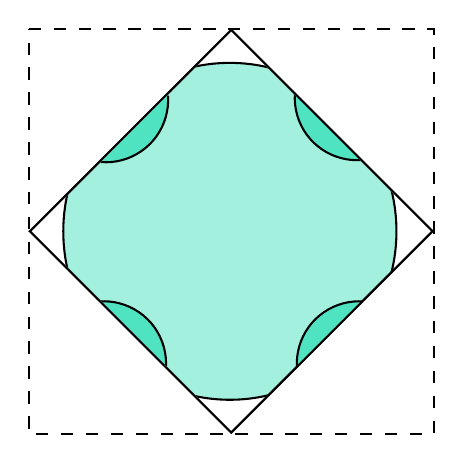
\begin{tikzpicture}[x=0.75pt,y=0.75pt,yscale=-1,xscale=1]
%uncomment if require: \path (0,300); %set diagram left start at 0, and has height of 300

%Shape: Path Data [id:dp6347441590753127] 
\draw  [fill={rgb, 255:red, 80; green, 227; blue, 194 }  ,fill opacity=0.52 ] (342.74,64.12) .. controls (349.21,64.12) and (355.5,64.9) .. (361.52,66.36) -- (420.58,125.41) .. controls (422.16,131.77) and (423,138.42) .. (423,145.28) .. controls (423,152.11) and (422.17,158.74) .. (420.6,165.07) -- (361.44,224.22) .. controls (355.44,225.67) and (349.18,226.44) .. (342.74,226.44) .. controls (336.93,226.44) and (331.25,225.81) .. (325.79,224.62) -- (264.46,163.3) .. controls (263.17,157.5) and (262.48,151.47) .. (262.48,145.28) .. controls (262.48,139.06) and (263.17,133) .. (264.48,127.19) -- (325.72,65.95) .. controls (331.2,64.75) and (336.9,64.12) .. (342.74,64.12) -- cycle ;
%Shape: Arc [id:dp9397326133788] 
\draw  [draw opacity=0][fill={rgb, 255:red, 80; green, 227; blue, 194 }  ,fill opacity=1 ] (406.41,110.91) .. controls (392.45,112.05) and (379.16,103.24) .. (375.16,89.25) .. controls (374.17,85.79) and (373.83,82.29) .. (374.07,78.89) -- (404,81) -- cycle ; \draw   (406.41,110.91) .. controls (392.45,112.05) and (379.16,103.24) .. (375.16,89.25) .. controls (374.17,85.79) and (373.83,82.29) .. (374.07,78.89) ;
%Shape: Square [id:dp49917369182880145] 
\draw   (343.42,48.25) -- (440.42,145.25) -- (343.42,242.25) -- (246.42,145.25) -- cycle ;
%Shape: Arc [id:dp8484610197939879] 
\draw  [draw opacity=0][fill={rgb, 255:red, 80; green, 227; blue, 194 }  ,fill opacity=1 ] (280.59,111.91) .. controls (294.55,113.05) and (307.84,104.24) .. (311.84,90.25) .. controls (312.83,86.79) and (313.17,83.29) .. (312.93,79.89) -- (283,82) -- cycle ; \draw   (280.59,111.91) .. controls (294.55,113.05) and (307.84,104.24) .. (311.84,90.25) .. controls (312.83,86.79) and (313.17,83.29) .. (312.93,79.89) ;
%Shape: Arc [id:dp6476837513798173] 
\draw  [draw opacity=0][fill={rgb, 255:red, 80; green, 227; blue, 194 }  ,fill opacity=1 ] (407.41,179.09) .. controls (393.45,177.95) and (380.16,186.76) .. (376.16,200.75) .. controls (375.17,204.21) and (374.83,207.71) .. (375.07,211.11) -- (405,209) -- cycle ; \draw   (407.41,179.09) .. controls (393.45,177.95) and (380.16,186.76) .. (376.16,200.75) .. controls (375.17,204.21) and (374.83,207.71) .. (375.07,211.11) ;
%Shape: Arc [id:dp5512282331487339] 
\draw  [draw opacity=0][fill={rgb, 255:red, 80; green, 227; blue, 194 }  ,fill opacity=1 ] (279.59,179.09) .. controls (293.55,177.95) and (306.84,186.76) .. (310.84,200.75) .. controls (311.83,204.21) and (312.17,207.71) .. (311.93,211.11) -- (282,209) -- cycle ; \draw   (279.59,179.09) .. controls (293.55,177.95) and (306.84,186.76) .. (310.84,200.75) .. controls (311.83,204.21) and (312.17,207.71) .. (311.93,211.11) ;
%Shape: Right Triangle [id:dp2444716275585217] 
\draw  [color={rgb, 255:red, 255; green, 255; blue, 255 }  ,draw opacity=1 ][fill={rgb, 255:red, 255; green, 255; blue, 255 }  ,fill opacity=1 ] (246.42,145.25) -- (343.42,48.25) -- (246.42,48.25) -- cycle ;
%Shape: Right Triangle [id:dp7467362132163622] 
\draw  [color={rgb, 255:red, 255; green, 255; blue, 255 }  ,draw opacity=1 ][fill={rgb, 255:red, 255; green, 255; blue, 255 }  ,fill opacity=1 ] (440.42,145.25) -- (343.42,48.25) -- (440.42,48.25) -- cycle ;
%Shape: Right Triangle [id:dp8978210412148069] 
\draw  [color={rgb, 255:red, 255; green, 255; blue, 255 }  ,draw opacity=1 ][fill={rgb, 255:red, 255; green, 255; blue, 255 }  ,fill opacity=1 ] (441,145.83) -- (344,242.83) -- (441,242.83) -- cycle ;
%Shape: Right Triangle [id:dp5172920566536954] 
\draw  [color={rgb, 255:red, 255; green, 255; blue, 255 }  ,draw opacity=1 ][fill={rgb, 255:red, 255; green, 255; blue, 255 }  ,fill opacity=1 ] (247,145.83) -- (344,242.83) -- (247,242.83) -- cycle ;
%Shape: Square [id:dp19483120370981322] 
\draw   (343.42,48.25) -- (440.42,145.25) -- (343.42,242.25) -- (246.42,145.25) -- cycle ;
%Shape: Square [id:dp47724188658303346] 
\draw  [dash pattern={on 4.5pt off 4.5pt}] (245.83,47.67) -- (441,47.67) -- (441,242.83) -- (245.83,242.83) -- cycle ;




\end{tikzpicture}
    }
    \subfigure[热点]{
        

\tikzset{every picture/.style={line width=0.75pt}} %set default line width to 0.75pt        

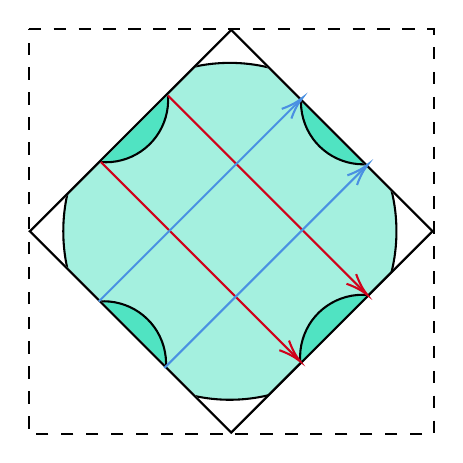
\begin{tikzpicture}[x=0.75pt,y=0.75pt,yscale=-1,xscale=1]
%uncomment if require: \path (0,300); %set diagram left start at 0, and has height of 300

%Shape: Path Data [id:dp28391475851762316] 
\draw  [fill={rgb, 255:red, 80; green, 227; blue, 194 }  ,fill opacity=0.52 ] (325.74,53.12) .. controls (332.21,53.12) and (338.5,53.9) .. (344.52,55.36) -- (403.58,114.41) .. controls (405.16,120.77) and (406,127.42) .. (406,134.28) .. controls (406,141.11) and (405.17,147.74) .. (403.6,154.07) -- (344.44,213.22) .. controls (338.44,214.67) and (332.18,215.44) .. (325.74,215.44) .. controls (319.93,215.44) and (314.25,214.81) .. (308.79,213.62) -- (247.46,152.3) .. controls (246.17,146.5) and (245.48,140.47) .. (245.48,134.28) .. controls (245.48,128.06) and (246.17,122) .. (247.48,116.19) -- (308.72,54.95) .. controls (314.2,53.75) and (319.9,53.12) .. (325.74,53.12) -- cycle ;
%Shape: Arc [id:dp4924996181571455] 
\draw  [draw opacity=0][fill={rgb, 255:red, 80; green, 227; blue, 194 }  ,fill opacity=1 ] (392.41,101.91) .. controls (378.45,103.05) and (365.16,94.24) .. (361.16,80.25) .. controls (360.17,76.79) and (359.83,73.29) .. (360.07,69.89) -- (390,72) -- cycle ; \draw   (392.41,101.91) .. controls (378.45,103.05) and (365.16,94.24) .. (361.16,80.25) .. controls (360.17,76.79) and (359.83,73.29) .. (360.07,69.89) ;
%Shape: Square [id:dp8258883831288684] 
\draw   (326.42,37.25) -- (423.42,134.25) -- (326.42,231.25) -- (229.42,134.25) -- cycle ;
%Shape: Arc [id:dp34996890506368183] 
\draw  [draw opacity=0][fill={rgb, 255:red, 80; green, 227; blue, 194 }  ,fill opacity=1 ] (263.59,100.91) .. controls (277.55,102.05) and (290.84,93.24) .. (294.84,79.25) .. controls (295.83,75.79) and (296.17,72.29) .. (295.93,68.89) -- (266,71) -- cycle ; \draw   (263.59,100.91) .. controls (277.55,102.05) and (290.84,93.24) .. (294.84,79.25) .. controls (295.83,75.79) and (296.17,72.29) .. (295.93,68.89) ;
%Shape: Arc [id:dp4561026088076878] 
\draw  [draw opacity=0][fill={rgb, 255:red, 80; green, 227; blue, 194 }  ,fill opacity=1 ] (392,164.96) .. controls (378.04,163.82) and (364.75,172.63) .. (360.75,186.61) .. controls (359.75,190.08) and (359.41,193.58) .. (359.65,196.97) -- (389.59,194.87) -- cycle ; \draw   (392,164.96) .. controls (378.04,163.82) and (364.75,172.63) .. (360.75,186.61) .. controls (359.75,190.08) and (359.41,193.58) .. (359.65,196.97) ;
%Shape: Arc [id:dp15892708580174042] 
\draw  [draw opacity=0][fill={rgb, 255:red, 80; green, 227; blue, 194 }  ,fill opacity=1 ] (262.59,168.09) .. controls (276.55,166.95) and (289.84,175.76) .. (293.84,189.75) .. controls (294.83,193.21) and (295.17,196.71) .. (294.93,200.11) -- (265,198) -- cycle ; \draw   (262.59,168.09) .. controls (276.55,166.95) and (289.84,175.76) .. (293.84,189.75) .. controls (294.83,193.21) and (295.17,196.71) .. (294.93,200.11) ;
%Shape: Right Triangle [id:dp9873621257073468] 
\draw  [color={rgb, 255:red, 255; green, 255; blue, 255 }  ,draw opacity=1 ][fill={rgb, 255:red, 255; green, 255; blue, 255 }  ,fill opacity=1 ] (229.42,134.25) -- (326.42,37.25) -- (229.42,37.25) -- cycle ;
%Shape: Right Triangle [id:dp20784307542005132] 
\draw  [color={rgb, 255:red, 255; green, 255; blue, 255 }  ,draw opacity=1 ][fill={rgb, 255:red, 255; green, 255; blue, 255 }  ,fill opacity=1 ] (423.42,134.25) -- (326.42,37.25) -- (423.42,37.25) -- cycle ;
%Shape: Right Triangle [id:dp19958209753051315] 
\draw  [color={rgb, 255:red, 255; green, 255; blue, 255 }  ,draw opacity=1 ][fill={rgb, 255:red, 255; green, 255; blue, 255 }  ,fill opacity=1 ] (424,134.83) -- (327,231.83) -- (424,231.83) -- cycle ;
%Shape: Right Triangle [id:dp13150240831757665] 
\draw  [color={rgb, 255:red, 255; green, 255; blue, 255 }  ,draw opacity=1 ][fill={rgb, 255:red, 255; green, 255; blue, 255 }  ,fill opacity=1 ] (230,134.83) -- (327,231.83) -- (230,231.83) -- cycle ;
%Shape: Square [id:dp6591394813744926] 
\draw   (326.42,37.25) -- (423.42,134.25) -- (326.42,231.25) -- (229.42,134.25) -- cycle ;
%Shape: Square [id:dp30244562238327477] 
\draw  [dash pattern={on 4.5pt off 4.5pt}] (228.83,36.67) -- (424,36.67) -- (424,231.83) -- (228.83,231.83) -- cycle ;
%Straight Lines [id:da43761852194250594] 
\draw [color={rgb, 255:red, 208; green, 2; blue, 27 }  ,draw opacity=1 ]   (295.93,68.89) -- (390.59,163.54) ;
\draw [shift={(392,164.96)}, rotate = 225] [color={rgb, 255:red, 208; green, 2; blue, 27 }  ,draw opacity=1 ][line width=0.75]    (10.93,-3.29) .. controls (6.95,-1.4) and (3.31,-0.3) .. (0,0) .. controls (3.31,0.3) and (6.95,1.4) .. (10.93,3.29)   ;
%Straight Lines [id:da018143618520460425] 
\draw [color={rgb, 255:red, 208; green, 2; blue, 27 }  ,draw opacity=1 ]   (263.59,100.91) -- (358.24,195.56) ;
\draw [shift={(359.65,196.97)}, rotate = 225] [color={rgb, 255:red, 208; green, 2; blue, 27 }  ,draw opacity=1 ][line width=0.75]    (10.93,-3.29) .. controls (6.95,-1.4) and (3.31,-0.3) .. (0,0) .. controls (3.31,0.3) and (6.95,1.4) .. (10.93,3.29)   ;
%Straight Lines [id:da48286677460832284] 
\draw [color={rgb, 255:red, 74; green, 144; blue, 226 }  ,draw opacity=1 ]   (262.59,168.09) -- (359.37,71.31) ;
\draw [shift={(360.79,69.89)}, rotate = 495] [color={rgb, 255:red, 74; green, 144; blue, 226 }  ,draw opacity=1 ][line width=0.75]    (10.93,-3.29) .. controls (6.95,-1.4) and (3.31,-0.3) .. (0,0) .. controls (3.31,0.3) and (6.95,1.4) .. (10.93,3.29)   ;
%Straight Lines [id:da3902094286940192] 
\draw [color={rgb, 255:red, 74; green, 144; blue, 226 }  ,draw opacity=1 ]   (294.21,200.11) -- (391,103.32) ;
\draw [shift={(392.41,101.91)}, rotate = 495] [color={rgb, 255:red, 74; green, 144; blue, 226 }  ,draw opacity=1 ][line width=0.75]    (10.93,-3.29) .. controls (6.95,-1.4) and (3.31,-0.3) .. (0,0) .. controls (3.31,0.3) and (6.95,1.4) .. (10.93,3.29)   ;




\end{tikzpicture}
    }
    \caption{布里渊区折叠和费米口袋形成}
\end{figure}

如果费米面和折叠后的第一布里渊区相交,费米面交叉处打开能隙,形成一系列小的费米口袋。热点附近的$\vb*{k}$和$\vb*{k} + \vb*{Q}$都在热点附近。

接下来讨论在热点附近的低能有效理论,换而言之,我们开始讨论超越平均场的物理。
需要注意的是考虑超越平均场的物理意味着将原本被忽略的涨落重新加入,这可能改变热点的位置或者甚至让热点消失(在本问题中不可能因为涨落不大,但确实有这样的体系,涨落会让平均场理论中出现的现象——如相变——消失,比如一维伊辛模型)。
因此,下面讨论的热点附近的低能有效理论建立在三个基础上:
\begin{enumerate}
    \item 费米面上存在热点,这是通过平均场理论算出来的,我们假定这个现象确实存在,而不是像一维伊辛模型一样只是幻象;
    \item 热点附近的低能有效理论是\eqref{eq:2dim-square-spin}的低能有效理论,即相互作用项一定是自旋-自旋相互作用(这并非假设,而是必然的事实);
    \item 低能自由度是低能电子和自旋波模式这两种场(实际上这是最重要的一个假设,因为低能自由度是什么通常难以直接计算得到)。
\end{enumerate}

\eqref{eq:2dim-square-spin}中的相互作用项是一个电子和一个自旋波模式(这是玻色子)发生散射,得到另一个电子,或者也可以说是自由电子的自旋和自旋波模式的相互作用。%
\footnote{自旋波模式是一部分形成了自旋波的电子被积掉之后得到的,和未形成自旋波长程序的电子是两群不同的电子。}%
因此低能有效理论的散射项形如%
\footnote{一个可能的问题是,为什么一定保留低能电子自由度和自旋波自由度?为什么不能是自旋波自由度和密度波自由度?不考虑自旋波-密度波自由度是因为没有明确的物理机制让这两个模式发生耦合,保留低能电子自由度是因为自旋算符和电子数算符对易,但和单个费米子算符并不对易,因此可能出现费米子自由度积不掉的情况。
这和BCS理论是不一样的,在BCS理论中大量电子参与配对,以至于哪怕电子自由度积不掉,它也不会产生太大作用。}%
\[
    {\phi}_{\vb*{q}} {c}^\dagger_{\vb*{k}+\vb*{q}\sigma} {c}_{\vb*{k}\sigma'},
\]
由于是低能有效理论,我们认为形成了一个基本上稳定的反铁磁序,于是$\vb*{q}$接近$\vb*{Q}$,而电子能量$\epsilon_{\vb*{k}}$和$\epsilon_{\vb*{k}+\vb*{q}}$都在费米面附近。
这些条件只有在热点附近才能达到。
当然由于热点是费米面交叠之后打开能隙的位置,在这附近有低能有效理论是非常合理的。
这样,一个散射过程涉及两个热点。分别用1和2标记两个热点,记它们的动量为$\vb*{K}_1$和$\vb*{K}_2$,则有
\[
    \vb*{K}_2 = \vb*{K}_1 + \vb*{Q},
\]
并重新定义$\vb*{q}$和$\vb*{k}$为它们偏离$\vb*{Q}$和$\vb*{K}_1$的大小。这样,相互作用哈密顿量就是
\[
    {\vb*{\phi}}_{\vb*{q}} \cdot (\sum_{\alpha, \beta} {c}^\dagger_{1(\vb*{k} + \vb*{q})\alpha} \vb*{\sigma}_{\alpha \beta} {c}_{2\vb*{k} \beta} + \text{h.c.}),
\]
这里任何一个散射过程中入射电子为热点1附加,出射电子在热点2附加或相反的原因是要保证所有电子的动量都在热点附加。于是完整的有效理论的哈密顿量为
\begin{equation}
    {H}_\text{eff} = \sum_{\vb*{k}, \sigma} (\xi_{1\vb*{k}} {c}^\dagger_{1\vb*{k} \sigma} {c}_{1 \vb*{k} \sigma} + \xi_{2\vb*{k}} {c}^\dagger_{2\vb*{k} \sigma} {c}_{2 \vb*{k} \sigma}) + {H}[\vb*{\phi}] + \lambda \sum_{\vb*{q}} {\vb*{\phi}}_{\vb*{q}} \cdot (\sum_{\alpha, \beta} {c}^\dagger_{1(\vb*{k} + \vb*{q})\alpha} \vb*{\sigma}_{\alpha \beta} {c}_{2\vb*{k} \beta} + \text{h.c.}).
    \label{eq:2dim-square-spin-eff}
\end{equation}
上式中没有明确提玻色场——也就是自旋波场——的自由哈密顿量。这个自由哈密顿量通常是通过对称性分析得出的。
进一步,由于是低能理论,将$\xi_{\vb*{k}}$在费米面附近做展开,仅保留一阶项,得到
\begin{equation}
    \xi_{1\vb*{k}} = \epsilon_{\vb*{k}} - \mu = \vb*{v}_1 \cdot \vb*{k}, \quad \xi_{2\vb*{k}} = \epsilon_{\vb*{k}} - \mu = \vb*{v}_2 \cdot \vb*{k}.
\end{equation}
使用$\vb*{v}_1$和$\vb*{v}_2$来标记$\grad_{\vb*{k}}{\xi_{\vb*{k}}}$是因为如果是自由电子气,那么它们就是费米速度。

\subsection{朗道阻尼}

现在我们尝试把电子完全积掉,只留下玻色型的自旋波模式。需要指出的是这个操作并不总是可行的:由于自旋波模式和电子都是低能自由度,简单地积掉其中一个自由度可能不能得到一个良定义的有效理论。
实际上,对二维体系的确会有这种棘手的细节。
下面的操作都是在默认确实可以积掉电子的前提下进行的。

从\eqref{eq:2dim-square-spin-eff}可以看出,一个自旋波模式可以衰变成一对电子空穴对,或者说一个自旋波模式可以将动量转移给一个电子而得到另一个电子,而自身湮灭。
因此自旋波模式是有有限的寿命的。由费米黄金法则,一个动量为$\vb*{q}$,能量为大于零的$\omega$的自旋波模式的寿命倒数为
\[
    \begin{aligned}
        \frac{1}{\tau} &\sim 2 \lambda^2 \int \frac{\dd[2]{\vb*{k}}}{(2\pi)^2} \delta(\omega + \epsilon_{1 \vb*{k}} - \epsilon_{2 (\vb*{k} + \vb*{q})}) \theta(- \epsilon_{1 \vb*{k}}) \theta(\epsilon_{2 (\vb*{k} + \vb*{q})}) \\
        &\sim \lambda^2 \int \frac{\dd{p_1} \dd{p_2}}{(2\pi)^2 \abs*{\vb*{v}_1 \times \vb*{v}_2}} \delta(\omega + p_1 - p_2) \theta(- p_1) \theta(p_2),
    \end{aligned}
\]
其中我们设
\[
    p_1 = \vb*{v}_1 \cdot \vb*{k}, \quad p_2 = \vb*{v}_2 \cdot (\vb*{k} + \vb*{q}),
\]
我们仅考虑低能理论,因此假定入射电子在费米面以下,出射电子在费米面以上。由几何关系,
\[
    \int \frac{\dd{p_1} \dd{p_2}}{\abs*{\vb*{v}_1 \times \vb*{v}_2}} \delta(\omega + p_1 - p_2) \theta(- p_1) \theta(p_2) = \sqrt{2} \omega,
\]
$\omega < 0$的情况也是一样的。总之最后自旋波模式的寿命为
\begin{equation}
    \frac{1}{\tau} \sim \frac{\lambda^2}{\abs*{\vb*{v}_1 \times \vb*{v}_2}} \abs*{\omega} = \gamma \abs*{\omega}.
\end{equation}
在格林函数中,衰变几率对应着自能修正,会直接反映在$\vb*{\phi}$的格林函数——从而有效作用量——中,也即,自旋波模式的推迟格林函数形如
\[
    G_{\vb*{\phi}}^{-1} = \ii \gamma \abs{\omega} + \cdots = \ii  \gamma \sgn(\omega) \omega + \cdots,
\]
相应的,松原格林函数形式为%
\footnote{这里的步骤是:先做Wick转动,即$\omega = \ii \omega_n$,}%
\[
    G_{\vb*{\phi}}^{-1} = \gamma \abs{\omega_n} + \cdots.
\]
这就意味着自旋波模式的有效热力学作用量为
\begin{equation}
    \begin{aligned}
        S_\text{eff} &= \sum_{\vb*{q}, \omega_n} \vb*{\phi}(-\vb*{q}, -\omega_n) \cdot (\gamma \abs{\omega_n} + \omega_n^2 + c^2 \vb*{q}^2 ) \vb*{\phi}(\vb*{q}, \omega_n) \\
        &= \sum_{\vb*{q}, \omega_n} \vb*{\phi}^*(\vb*{q}, \omega_n) \cdot (\gamma \abs{\omega_n} + \omega_n^2 + c^2 \vb*{q}^2) \vb*{\phi}(\vb*{q}, \omega_n).
    \end{aligned}
    \label{eq:effective-spin-action}
\end{equation}
第二个等号是因为$\vb*{\phi}$是实场,因为负的动量/频率等价于取复共轭。
$\omega_n^2$项和$\vb*{q}^2$项都是对称性分析加入的项,除此以外的项在低能有效理论中并不重要。%
$\omega_n^2$项和$\vb*{k}^2$项可以容易地切换到实空间,它们分别对应着时间导数平方项$(\partial_\tau \phi)^2$和梯度平方项$(\grad{\phi})^2$,但$\abs{\omega_n}$在实空间中没有简单的形式。
不过,一个正比于$\omega_n$的项意味着实空间中有某种阻尼,这也是正确的,因为自旋波模式如前所述会衰变。这种阻尼或者衰变称为\concept{朗道阻尼}。朗道阻尼指的是没有粒子之间的相互碰撞,仅仅粒子和波强烈耦合也能够产生阻尼。

\subsection{RPA近似计算朗道阻尼}

还可以通过直接计算格林函数的方式来得到$\phi$的有效理论。
这个有效理论当然取
\[
    Z_\text{eff} = \int \mathcal{D}\vb*{\phi} \ee^{- \sum_{q, \omega_n} \vb*{\phi}^*(\vb*{q}, \omega_n) G^{-1}_{\vb*{\phi}}(\vb*{q}, \omega_n) \vb*{\phi}(\vb*{q}, \omega_n)}
\]
的形式。

\subsection{Hertz理论}

最后我们讨论上一节得到的低能有效理论的

\subsection{RPA近似}

我们尝试对平均场近似做一些修正。为此我们将不再直接处理自旋算符,而是把一切都转化到费米子算符上。
做傅里叶变换
\[
    {S}_{\vb*{q}} = \frac{1}{\sqrt{N_\text{site}}} \sum_{\vb*{i}} {S}_i \ee^{\ii \vb*{r}_i \cdot \vb*{q}} = \frac{1}{\sqrt{N_\text{site}}} \sum_{\vb*{k}} {c}^\dagger_{\vb*{k}+\vb*{q}, \alpha} \vb*{\sigma}_{\alpha \beta} {c}_{\vb*{k} \beta},
\]
这样相互作用项就是(请注意$\vb*{\sigma}$)

对相互作用项做正规序不会影响定性的结果,我们不需要动手算就知道正规序和原本的相互作用只会差一个单体项,而这个单体项是自选旋转不变的,那么它只会对$\epsilon_{\vb*{k}} - \mu$做一个修正。
于是我们将要处理以下相互作用哈密顿量:% TODO:自旋
\begin{equation}
    {H} = \frac{1}{2 N_\text{site}} \sum_{\vb*{k}, \vb*{k}', \vb*{q}, \alpha, \beta} {c}^\dagger_{\vb*{k}-\vb*{q}, \alpha} {c}^\dagger_{\vb*{k}'+\vb*{q}, \beta} V(\vb*{q}) {c}_{\vb*{k}'} {c}_{\vb*{k}}, \quad V(\vb*{q}) = 2 J (\cos(q_x) + \cos(q_y)).
\end{equation}

\begin{equation}
    Z = \int \fd{\vb*{\phi}} \exp(- \int_0^\beta \dd{\tau} )
\end{equation}

$\vb*{\phi}$就像驱动自旋的一个外场一样,在只取鞍点近似时它就是平均场序参量。

\section{local repulsion导致的反铁磁长程序}

前一节讨论的模型中的反铁磁序能够形成是因为我们塞入了一个能够形成反铁磁序的哈密顿量。
实际上,如果模型中没有显式的自旋-自旋相互作用,最后可能也是能够形成一个反铁磁序的。
本节研究二维正方格子上的如下模型:
\begin{equation}
    H = - t \sum_{\pair{\vb*{i}, \vb*{j}}, \alpha} t (c^\dagger_{\vb*{i} \alpha} c_{\vb*{j} \alpha} + \text{h.c.}) - \mu N + U \sum_{\vb*{i}} n_{\vb*{i}}^2,
\end{equation}
其自由理论部分就是一个典型的紧束缚模型,其能谱为
\begin{equation}
    \xi_{\vb*{k}} = - 2t (\cos(k_x a) + \cos(k_y a)) - \mu.
\end{equation}

这个模型基本上是Hubbard模型去掉自旋依赖的版本。
它在低温下可能能够产生CDW序或是SDW序。它能够产生什么序可以通过仿照BCS超导,通过计算相应的序参量的关联函数得到。

